% IOE BE Project Latex Template by Santosh Giri, Assistant Professor, DOECE, Pulchowk Campus, IOE, TU
\documentclass[12pt]{report}
\usepackage{xcolor}
\usepackage[utf8]{inputenc}
\usepackage{fontspec}
\newfontfamily\devanagarifont{Noto Sans Devanagari} 

\usepackage{graphicx}
\usepackage{booktabs}
\usepackage{float}
\usepackage{caption}
\usepackage{subcaption}
\usepackage{array}
\usepackage{multirow}
\usepackage{amsmath}
\usepackage{natbib}%referencing
\usepackage[left=1.0in,right=1.0in,top=.8in,bottom=.8in]{geometry}
\usepackage{float}
\usepackage{tikz} %for diagrams
\usepackage{subcaption} % in preamble
\usepackage{pgfgantt}
\usetikzlibrary{shapes.geometric, arrows, positioning, fit, backgrounds}
\usepackage{hyperref} %for clickable links\usepackage{hyperref} %for clickable links

\newfontfamily\nepalifont{Noto Serif Devanagari}
\linespread{1.3}
\usepackage{graphicx}%figures
\usepackage{rotating}%landscape
\usepackage{amsmath}%math
\usepackage{titlesec} %formatting chapters
%\titlespacing*{<command>}{<left>}{<before-sep>}{<after-sep>}
\titlespacing*{\chapter}{-15pt}{10pt}{15pt}
\titlespacing*{\section}{0pt}{0pt}{5pt}
\titlespacing*{\subsection}{0pt}{5pt}{5pt}
\titleformat{\chapter}[hang] 
{\normalfont\huge\bfseries}{\chaptertitlename\ \thechapter.}{1em}{}
\renewcommand{\chaptername}{}
\graphicspath{{Images/}}%image folder name
%Cover page contents
\title{
{
\includegraphics[scale=.3]{logotu.jpg}}\\
\uppercase\large{
    {Tribhuvan University}\\
    {Institute of Engineering}\\
    {Pulchowk Campus}\\
    \vspace{.5cm}
    {A \\Project Report\\On\\SajiloText - Simplifying Complex Nepali Language Using AI}\\
    \vspace{.5cm}
    {\textbf{Submitted By:}\\Bishal Babu Bhattarai (PUL078BEI013) \\MANORATH BHATT (PUL078BEI021) \\SALIZ THAPA (PUL078BEI033)}\\
    \vspace{.5cm}
    {\textbf{Submitted To:}\\ Department of Electronics \& Computer engineering}\\
                }
    }
   
\date{\today} %{Month Year}
\begin{document}
\maketitle
\pagenumbering{roman}
\setcounter{page}{2}

\newpage   


\chapter*{Page of Approval}
\addcontentsline{toc}{chapter}{\numberline{}Page of Approval}
\thispagestyle{empty}

\vspace*{1.2cm}

\begin{center}
    \textbf{TRIBHUVAN UNIVERSITY}\\
    \textbf{INSTITUTE OF ENGINEERING}\\
    \textbf{PULCHOWK CAMPUS}\\
    \textbf{DEPARTMENT OF ELECTRONICS AND COMPUTER ENGINEERING}
\end{center}

\vspace{1.2cm}

\noindent
The undersigned certifies that they have read and recommended to the Institute of Engineering for acceptance of a project report entitled
\textbf{``SAJILOTEXT - SIMPLIFYING COMPLEX NEPALI LANGUAGE USING AI''}
submitted by \textbf{Bishal Babu Bhattarai, Manorath Bhatt and Saliz Thapa}
in partial fulfillment of the requirements for the Bachelor's degree in Electronics, Communication \& Information Engineering.

\vspace{1.2cm}

\noindent
\begin{minipage}[t]{0.45\textwidth}
    \raggedright
    \rule{4cm}{0.4pt}\\
    Supervisor\\[0.2cm]
    \textbf{Asst Prof. Anku Jaiswal}\\
    Department of Electronics and Computer
    Engineering,\\
    Pulchowk Campus, IOE, TU.
\end{minipage}
\hfill
\begin{minipage}[t]{0.45\textwidth}
    \raggedleft
    \rule{4cm}{0.4pt}\\
    Internal examiner\\[0.2cm]
    Department of Electronics and Computer
    Engineering,\\
    Pulchowk Campus, IOE, TU.
\end{minipage}

\vspace{1.2cm}

\begin{center}
    \rule{4cm}{0.4pt}\\
    External examiner\\[0.2cm]
    Department of Electronics and Computer Engineering,\\
    Pulchowk Campus, IOE, TU.
\end{center}

\vspace{0.8cm}

\begin{center}
    Date of approval:
\end{center}


\chapter*{Acknowledgments}
\addcontentsline{toc}{chapter}{\numberline{}Acknowledgements}

We would like to express our heartfelt gratitude to all those who have supported and guided us throughout the preparation and development of our major project proposal titled \textbf{"SAJILOTEXT - SIMPLIFYING COMPLEX NEPALI LANGUAGE USING AI"}. First and foremost, We are deeply thankful to our respected project supervisor, \textbf{Assistant professor Anku Jaiswal}, for her constant support, valuable feedback, and insightful guidance at every stage of the project. Her mentorship has been instrumental in shaping our ideas and refining our project. We also extend our sincere thanks to the Department of Electronics and Computer Engineering, Pulchowk Campus, for providing us with the platform and resources to pursue this project. The academic environment and support from faculty members have greatly contributed to our progress. We appreciate the encouragement and collaboration from our fellow classmates and friends, whose discussions and suggestions have helped us think critically and improve our approach. Lastly, we are thankful to our families for their continuous encouragement, patience, and support, which have kept us motivated throughout this journey. We look forward to continuing our project with dedication and a strong sense of responsibility toward addressing real-world language accessibility challenges.\vspace{2 cm} \\ BISHAL BABU BHATTARAI (PUL078BEI013)\\
MANORATH BHATT (PUL078BEI021)\\
SALIZ THAPA (PUL078BEI033)

\newpage
\chapter*{Abstract}
\addcontentsline{toc}{chapter}{\numberline{}Abstract}
This project presents the implementation of a Nepali legal text simplification system using the multilingual Transformer model mT5. The primary objective of the proposed approach is to transform complex Nepali legal text into simpler and more understandable Nepali while preserving the original legal meaning. The system is designed to assist ordinary readers in understanding difficult legal provisions, particularly those written in formal constitutional and legal language.

The project consists of several stages, including dataset collection, data cleaning and preprocessing, preparation of parallel complex–simple Nepali text pairs, and fine-tuning of the mT5 model for the simplification task. The dataset is developed from Nepali legal texts(Constitution and the Social Studies text books) and manually refined to ensure that the simplified outputs are shorter, clearer, and easier to understand without losing the core meaning of the original text. To verify the quality of the dataset, Lexical Complexity Analysis and the Sari Score Analysis is performed. The trained model is evaluated using automatic evaluation metrics such as BLEU and ROUGE scores, along with qualitative examination of output clarity and meaning preservation.

The proposed approach demonstrates the potential of Transformer-based models for Nepali legal text simplification. It provides a practical solution for generating simpler versions of legal content that can be useful for citizens, students, and readers with limited legal literacy. In addition, the project highlights the importance of high-quality parallel datasets and suitable preprocessing methods in improving the performance of simplification models for low-resource legal language tasks.

In conclusion, this work shows that fine-tuning mT5 for Nepali legal text simplification is a promising direction for making legal information more accessible and understandable, while also contributing a foundation for future research in Nepali legal natural language processing.

Keywords: mT5, Nepali Legal Text Simplification, Transformers, Low-Resource Language Processing, Lexical Complexity Analysis, Sari Score Analysis, BLEU Score, ROUGE Score, Legal NLP

\tableofcontents
\addcontentsline{toc}{chapter}{\numberline{}Table of Contents}
\listoffigures
\addcontentsline{toc}{chapter}{\numberline{}List of Figures}
% \listoftables
% \addcontentsline{toc}{chapter}{\numberline{}List of Tables}
\chapter*{List of Abbreviations}
\addcontentsline{toc}{chapter}{\numberline{}List of Abbreviations}
\begin{tabular}{c l}
\textbf{AI}     &  Artificial Intelligence\\
\textbf{NLP}    &  Natural Language Processing\\
\textbf{ATS}    &   Automated Text Simplification\\
\textbf{BERT}   &  Bidirectional Encoder Representations from Transformers \\
\textbf{RoBERTa}& Robustly Optimized BERT Pretraining Approach\\
\textbf{OCR}    &Optical Character Recognition\\
\textbf{LLM}    &Large Language Models\\
\textbf{CNN}    &Convolutional Neural Network\\
\textbf{JSON}   &  JavaScript Object Notation\\
\textbf{ROUGE}  &  Recall-Oriented Understudy for Gisting Evaluation\\
\textbf{API}    &  Application Programming Interface\\
\textbf{GPU}    &  Graphics Processing Unit\\
\textbf{BLEU}    &  Bilingual Evaluation Understudy\\
\textbf{mT5}     &  Massively Multilingual Pre-trained Text-to-Text Transformer\\
\textbf{SARI}    &  System output Against References and against the Input\\
\\



\end{tabular}

% instruction ends here
\chapter{Introduction}
\pagenumbering{arabic}%start arabic numbering(1,2,3..) from here
\section{Background}
In Nepali schools, subjects like Civic Sense and The Constitution help students learn about their rights, duties, and how the government works. These subjects are meant to build responsible and informed citizens. But the problem is that the language used in these textbooks is often very formal and difficult. Many students, who are used to reading and speaking in everyday Nepali, find it hard to understand. Because of this, they end up memorizing the lessons instead of really learning what they mean.

Today, with the help of AI and NLP, it is possible to make such difficult texts easier to read. The SajiloText Project is designed to do exactly that. It uses AI tools to simplify complex Nepali texts from Civic Sense lessons, the Constitution, and other legal documents. The system makes sentences shorter and clearer, replaces hard words with simpler ones, and even provides easy English translations and word meanings.

By doing this, SajiloText works like a digital learning helper. It helps students truly understand their lessons instead of just memorizing them. The goal of this project is to make civic education more interesting, easier to learn, and more accessible for all Nepali students.
\section{Problem statements}
Many official, legal, and educational documents in Nepali are written in complex and formal language, making them difficult for students and general readers to understand. This creates a barrier to effective learning and access to important information. Existing translation tools do not accurately simplify Nepali text or capture the true meaning in context. Moreover, there is a lack of AI-based systems specifically designed to simplify Nepali language content. As a result, readers- especially students often rely on memorization instead of genuine understanding, leading to poor learning outcomes and reduced interest in reading.
\section{Objectives}
 The primary objectives of our project SajiloText are as follows:
\begin{itemize}
\item Build a tool that simplifies Nepali lessons from the Civic Sense chapters of Class 8-10 and the Constitution. 

\item Detect hard words and give simple meanings or examples.
\item Use OCR to read Nepali text from images or scanned pages.
\item Create an easy-to-use web app for students and teachers.
\end{itemize}
\section{Scope}
The SajiloText Project aims to develop an AI-based system that simplifies complex Nepali texts from Civic Sense lessons, the Constitution of Nepal, and related legal documents. The system will make difficult words and sentences easier to understand, and explain key terms. This project focuses on helping students in Classes 8–10 and general readers better comprehend educational materials. It does not change the original content but makes it more accessible through AI-powered text simplification tools.
\chapter{Literature Review}
The field of ATS holds immense potential for enhancing information accessibility, a challenge that is particularly acute for low-resource languages which lack the vast, structured digital corpora that fuel modern AI development. Nepali squarely falls into this category; despite being spoken by millions, its digital footprint in the form of machine-readable datasets is limited, posing a significant barrier to the advancement of sophisticated Natural Language Processing (NLP) tools. This data scarcity directly impacts crucial applications where clarity is paramount, most notably in educational accessibility, where students often struggle to comprehend the formal language of textbooks, and in legal comprehension, where citizens may find it difficult to understand official documents. A review of the current landscape in Nepali NLP reveals that research efforts have predominantly focused on foundational tasks such as text classification, sentiment analysis, and, with growing interest, machine translation. While these are vital areas, they have left other critical applications underdeveloped. The advent of powerful transformer architectures like BERT, RoBERTa, and GPT-2 has revolutionized NLP by enabling models to grasp deep contextual nuances, offering a promising technological foundation for tackling more complex linguistic challenges. However, a significant gap in Nepali text simplification research remains, with a distinct lack of dedicated models or publicly available systems designed to make complex Nepali texts more understandable. Recognizing that the primary obstacle is the absence of a large-scale parallel corpus (complex-simple sentence pairs), this project addresses the problem at its root through the manual curation of a high-quality, domain-specific dataset. This approach serves as a practical solution to the corpus shortage, providing the necessary foundation to fine-tune a state-of-the-art model specifically for the task of simplifying educational content for Nepali students.
\section{Related work}
Text simplification is an active area of natural language processing (NLP) research with applications in accessibility, education, legal communication, and cross-linguistic information retrieval. This section reviews the most significant prior works that influenced the design of SajiloText, organized by research theme.

\subsection*{Text Simplification for High-Resource Languages}
The majority of early work in automatic text simplification focused on English, leveraging large parallel corpora such as Simple English Wikipedia paired with standard Wikipedia. Zhu et al. (2010) proposed one of the first statistical machine translation (SMT) approaches to text simplification, treating the task as a monolingual translation problem from complex to simple language. Their tree-based model enabled sentence splitting, deletion of non-essential clauses, and lexical substitution.
Subsequent work by Wubben et al. (2012) demonstrated that phrase-based SMT systems trained on Wikipedia-SimpleWikipedia pairs could outperform rule-based approaches on readability metrics. Xu et al. (2016) introduced the Newsela corpus — a professionally edited parallel corpus of news articles at multiple reading levels — which significantly improved dataset quality and model training outcomes.
The advent of neural sequence-to-sequence models marked a turning point. Nisioi et al. (2017) applied encoder-decoder LSTMs with attention mechanisms to text simplification and demonstrated competitive performance against SMT baselines. Later, Dong et al. (2019) introduced controllable text simplification where a model could be conditioned on specific simplicity levels, enabling graduated outputs for different reader populations.
\subsection{Transformer-Based Simplification Models} 
The introduction of the Transformer architecture (Vaswani et al., 2017) and subsequent pre-trained language models (PLMs) fundamentally transformed text simplification. BERT (Devlin et al., 2019) demonstrated that models pre-trained on large unlabelled corpora using masked language modelling could be fine-tuned for downstream NLP tasks with minimal task-specific data.
For text generation tasks including simplification, encoder-decoder Transformer models proved most effective. T5 (Raffel et al., 2020) reframed all NLP tasks as text-to-text transformations — an approach closely mirrored in SajiloText through the use of the task prefix 'simplify Nepali: ' that conditions the model on the simplification objective. Martin et al. (2020) proposed ACCESS — a controllable Simplification model based on BART — which allowed explicit control over sentence length, lexical complexity and paraphrase rate, achieving state-of-the-art SARI scores on English benchmarks.
Sheang and Saggion (2021) conducted a comprehensive evaluation of pre-trained models including T5, BART, and GPT-2 for automated text simplification, finding that T5-based models consistently outperformed alternatives on both automatic metrics (BLEU, SARI) and human evaluation criteria (grammaticality, simplicity, adequacy).
\subsection{Multilingual and Low-Resource Text Simplification}
Research on text simplification for languages other than English remains considerably limited, primarily due to the scarcity of parallel corpora. Notable exceptions include work on Spanish (Saggion et al., 2015), Portuguese (Scarton and Specia, 2018), Italian (Brunato et al., 2015), and German (Sauberli et al., 2020).
For truly low-resource languages, transfer learning from multilingual pre-trained models has emerged as the dominant approach. Multilingual BERT (mBERT) and its successor XLM-RoBERTa demonstrated that cross-lingual representations learned on 100+ languages could be adapted to low-resource downstream tasks. However, these models are primarily encoder-only and cannot directly generate simplified text.
mT5 (Xue et al., 2021), the multilingual variant of T5, addressed this gap by pre-training a text-to-text Transformer on the mC4 corpus — a 101-language web crawl. mT5 supports Nepali natively in its vocabulary and was pre-trained on Nepali web text, making it the most suitable off-the-shelf model for fine-tuning on Nepali legal text simplification. This forms the primary motivation for SajiloText's architectural choice of mT5-small as the base model.
\subsection{Legal Text Simplification}
Legal documents present unique challenges for text simplification due to their specialized vocabulary, complex syntactic structures, nested clause hierarchies, and the requirement that simplified outputs remain legally accurate. Marino et al. (2019) demonstrated that standard simplification systems trained on Wikipedia data performed poorly on legal text without domain-specific fine-tuning.
Specifically for legal text, Chalkidis et al. (2020) introduced the LegalBERT model- a domain-adapted BERT pre-trained on legal corpora- and showed substantial improvements on legal NLP tasks over general-purpose models. Whilst LegalBERT targets understanding rather than generation, the domain adaptation principle directly informs SajiloText's approach of fine-tuning on domain-specific Nepali legal pairs rather than using a general-purpose model zero-shot.
For the Nepali legal domain specifically, prior computational work is essentially absent from published literature. The Nepal Law Commission website and the Supreme Court of Nepal provide legal documents exclusively in formal written Nepali, but no academic system for automatically simplifying these documents has been published prior to this work.
\subsection{Nepali Natural Language Processing} 
Nepali is a morphologically rich Indo-Aryan language written in Devanagari script with approximately 17 million native speakers. Despite its linguistic complexity, published NLP research in Nepali remains sparse compared to major world languages.
Key prior works include: Bal and Rupakheti (2010) who developed the Nepali National Corpus; Pandey (2014) who built a Nepali POS tagger; Shahi and Pant (2018) who evaluated neural sentiment analysis for Nepali social media text; and Bhattarai et al. (2022) who applied multilingual BERT to Nepali question answering.
In the area of machine translation, several works have addressed Nepali-English neural machine translation. Duwal and Bal (2019) demonstrated that standard seq2seq models with attention produced reasonable Nepali-English translations, and subsequent work leveraged mBERT and XLM-R for improved cross-lingual transfer.
For text generation specifically, Nepali NLP faces three compounding challenges: (1) the relatively small Nepali pre-training corpus in models like mT5, (2) the agglutinative morphology of Nepali that makes word-level tokenization suboptimal, and (3) the use of Devanagari script which requires Unicode-aware processing throughout the pipeline. SajiloText addresses all three challenges through character-level BLEU evaluation, sentencepiece-based subword tokenization inherited from mT5, and Devanagari-aware post-processing in the web application backend.

\section{Related Theory}

This project is grounded in the theory of natural language processing, deep learning, sequence-to-sequence generation, and multilingual Transformer models. Since the objective is to convert complex Nepali legal text into simpler Nepali while preserving legal meaning, the theoretical foundation must explain how text is represented, how neural models learn mappings between complex and simple sentences, how Transformer architectures model long legal clauses, and how preprocessing ensures the quality of the dataset used for fine-tuning. The following subsections describe the theoretical concepts most relevant to the proposed Nepali legal text simplification system.

\subsection{Language Representation}

Language representation is the process of transforming raw text into a numerical form that can be processed by a machine learning model. Since a neural model cannot directly interpret words, each sentence must be converted into tokens, vectors, or embeddings before learning can occur. In natural language processing, this representation stage is critical because it determines how much semantic, syntactic, and contextual information is available to the model.

Early approaches to text representation were based on one-hot encoding and bag-of-words models. In one-hot encoding, each word in a vocabulary of size $|V|$ is represented by a vector $\mathbf{x}_i \in \mathbf{R}^{|V|}$ in which only one position is $1$ and all others are $0$:

\begin{equation}
\mathbf{x}_i = [0,0,\dots,1,\dots,0]^T
\end{equation}

Although this method uniquely identifies a word, it does not capture semantic similarity. Two related words receive two completely different vectors even if they are close in meaning. Likewise, bag-of-words models represent a sentence or document by counting word occurrences, but they ignore word order and context. Such representations are weak for legal language, where meaning often depends on the relationship between specific terms and the order in which conditions and exceptions appear.

Dense embeddings improved this limitation by mapping tokens into a continuous vector space. Let $E \in \mathbf{R}^{|V| \times d}$ be an embedding matrix, where $d$ is the embedding dimension. The embedding of token $i$ is:

\begin{equation}
\mathbf{e}_i = E^T \mathbf{x}_i
\end{equation}

In this representation, semantically related words tend to lie closer in the vector space. However, static embeddings still assign one fixed representation to a word, regardless of its context. In legal language, this is often insufficient. Words such as {\devanagarifont अधिकार}, {\devanagarifont प्रतिबन्ध}, and {\devanagarifont बमोजिम} may carry different practical force depending on the sentence in which they appear.

Modern Transformer-based models solve this by learning \textbf{contextual language representations}. Instead of assigning a single fixed vector to each token, the model computes a context-sensitive representation using all other tokens in the sentence. This is especially important in legal simplification, where the meaning of the sentence can depend heavily on conditions such as {\devanagarifont तर}, {\devanagarifont बाहेक}, {\devanagarifont यस ऐन बमोजिम}, or {\devanagarifont अन्यथा व्यवस्था भएमा}. These terms cannot simply be removed or replaced without understanding their contextual role.

Another important theoretical aspect of this project is \textbf{subword tokenization}. Nepali is morphologically rich, and legal texts contain many rare compounds, formal expressions, and low-frequency words. Word-level tokenization therefore leads to many unknown or very sparse tokens. To address this, the mT5 model uses SentencePiece-based subword tokenization. A sentence $S$ is decomposed into a sequence of subword tokens:

\begin{equation}
S = \{t_1, t_2, t_3, \dots, t_n\}
\end{equation}

This allows the model to handle rare legal forms more effectively. For example, a long word or phrase does not need to be memorized as a single vocabulary item if it can be split into meaningful smaller units. This greatly improves robustness in Nepali legal NLP.

In the proposed project, language representation is therefore implemented in the following pipeline:
\begin{enumerate}
    \item raw Nepali legal text is segmented into tokens or subwords,
    \item each token is converted to an ID,
    \item token IDs are mapped to dense vectors,
    \item contextual representations are learned through the Transformer encoder,
    \item the decoder generates a simplified Nepali sentence from these contextual features.
\end{enumerate}

Thus, language representation is not merely a preprocessing step; it is the foundation that allows the model to understand legal structure, preserve meaning, and generate simpler expression.

\begin{figure}[H]
    \centering
    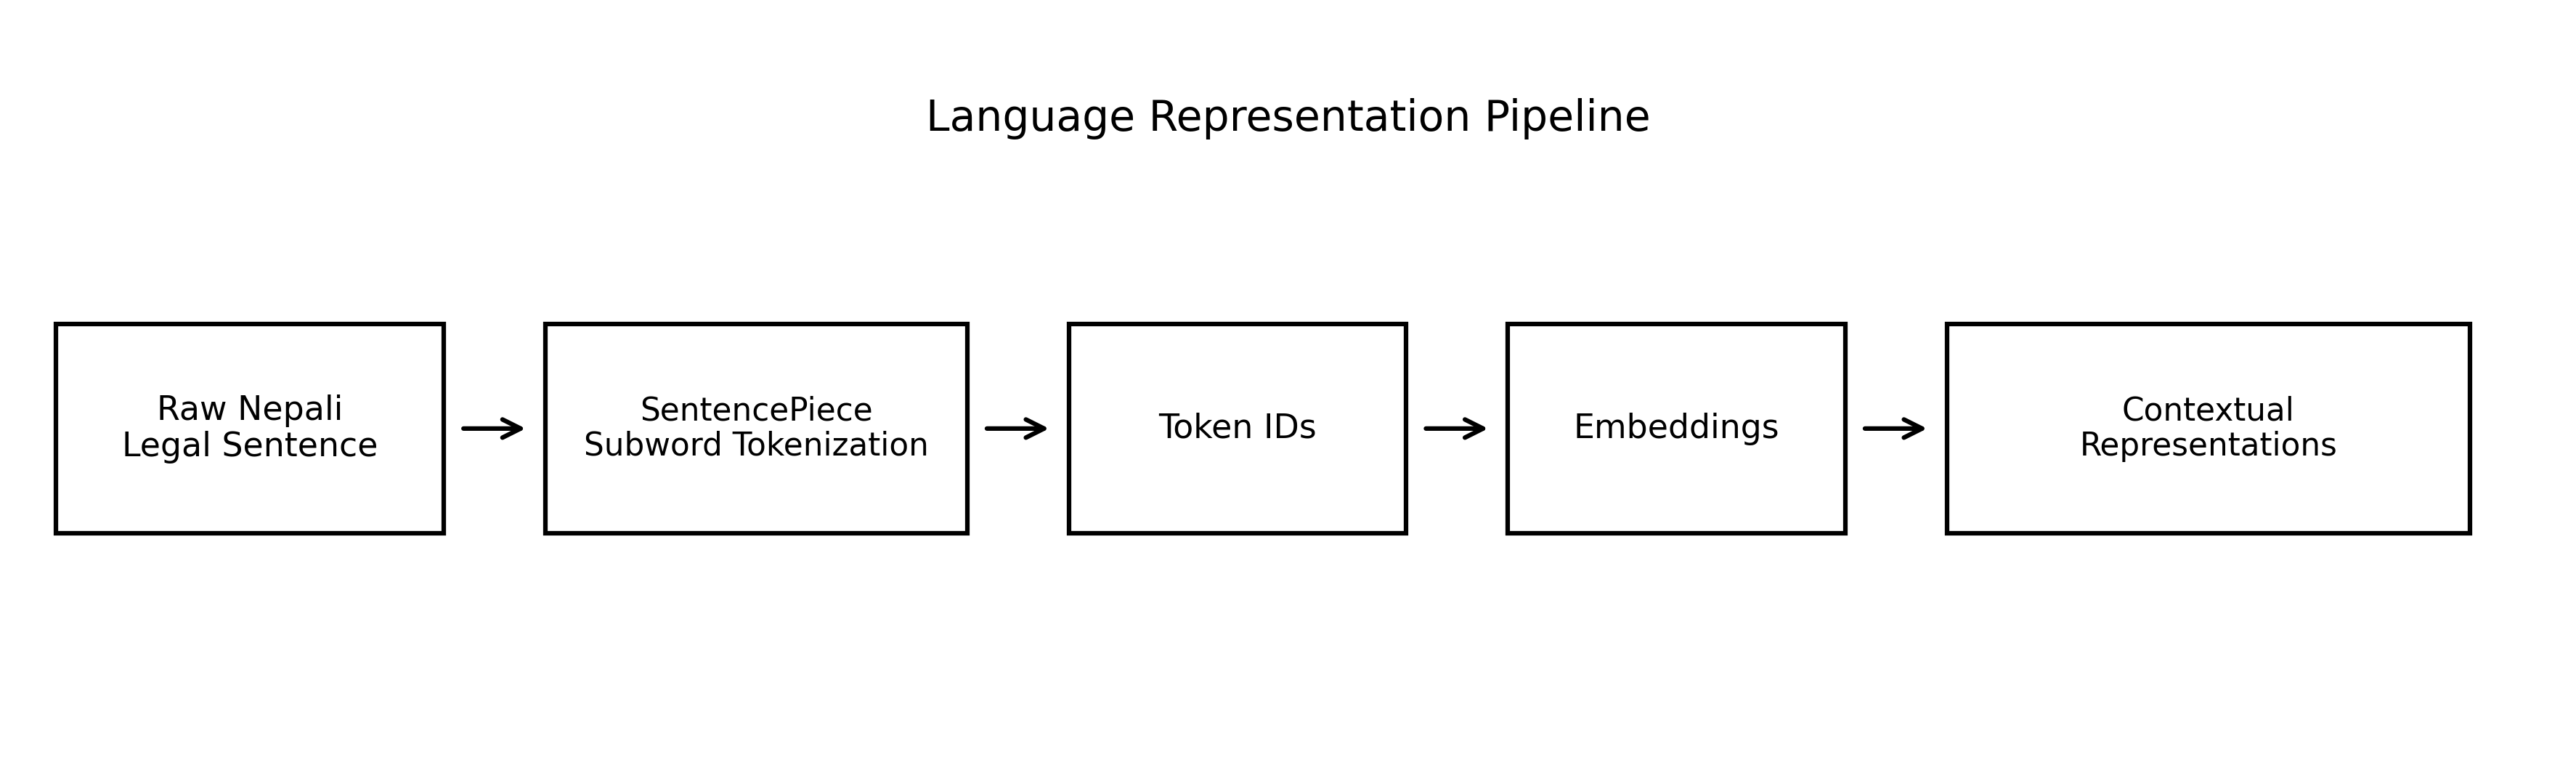
\includegraphics[width=0.92\textwidth]{language_representation_pipeline_fixed.png}
    \caption{Language representation pipeline for Nepali legal text simplification: raw sentence, subword tokenization, token IDs, embeddings, and contextual representations.}
    \label{fig:language_representation}
\end{figure}

\subsection{Neural Networks}

Neural networks are the learning engine behind modern NLP systems. A neural network consists of layers of computational units called neurons. Each neuron receives inputs, applies weights and a bias, and passes the result through a nonlinear activation function. For a neuron with input vector $\mathbf{x}$, weight vector $\mathbf{w}$, and bias $b$, the output is:

\begin{equation}
z = \mathbf{w}^T \mathbf{x} + b
\end{equation}

\begin{equation}
a = \phi(z)
\end{equation}

where $\phi(\cdot)$ is an activation function such as ReLU, tanh, or sigmoid.

In text generation tasks, the model must learn a mapping from an input sequence to an output sequence. This led to the development of \textbf{sequence-to-sequence} neural models. In such models, an encoder reads the input sentence and compresses it into internal representations, while a decoder generates the target sentence token by token. The conditional probability of generating a target sentence $\mathbf{y} = (y_1, y_2, \dots, y_T)$ from a source sentence $\mathbf{x}$ is:

\begin{equation}
P(\mathbf{y} \mid \mathbf{x}) = \prod_{t=1}^{T} P(y_t \mid y_{<t}, \mathbf{x})
\end{equation}

This equation means that the next output token depends on the input sentence and all previously generated output tokens.

Earlier neural simplification models used recurrent neural networks, long short-term memory networks, or gated recurrent units. These models improved over rule-based simplification, but they often struggled with long-range dependencies. This weakness is significant in legal text, where the condition that governs the entire sentence may appear many tokens before the main verb or obligation.

Training a neural network requires a loss function and an optimization procedure. In this project, the model is trained using token-level cross-entropy loss between the generated output and the target simplified sentence:

\begin{equation}
\mathcal{L} = - \sum_{t=1}^{T} \log P(y_t^{*} \mid y_{<t}^{*}, \mathbf{x})
\end{equation}

where $y_t^{*}$ is the correct target token at time step $t$. The objective is to minimize this loss over the training dataset.

During backpropagation, gradients of the loss with respect to model parameters are computed and used to update the weights. If $\theta$ denotes the set of trainable parameters, a gradient-based update has the general form:

\begin{equation}
\theta \leftarrow \theta - \eta \nabla_{\theta}\mathcal{L}
\end{equation}

where $\eta$ is the learning rate. If the learning rate is too high, the model may become unstable; if it is too low, learning becomes excessively slow. Since this project uses a relatively small custom Nepali legal dataset, careful parameter tuning is essential.

To improve generalization, the model also relies on regularization techniques. Common methods include weight decay, dropout, and early stopping. Dropout randomly suppresses some units during training:

\begin{equation}
\tilde{\mathbf{h}} = \mathbf{m} \odot \mathbf{h}
\end{equation}

where $\mathbf{m}$ is a binary mask sampled from a Bernoulli distribution and $\odot$ denotes element-wise multiplication. Such regularization is particularly important for legal simplification, because a model trained on limited data can easily memorize sentence patterns instead of learning robust rewriting behavior.

In this project, the network is not trained from scratch. Instead, a pretrained multilingual model is \textbf{fine-tuned}. Fine-tuning transfers broad multilingual language knowledge into the domain of Nepali legal simplification. This is both computationally practical and more effective than building a model from the beginning.

\begin{figure}[H]
    \centering
    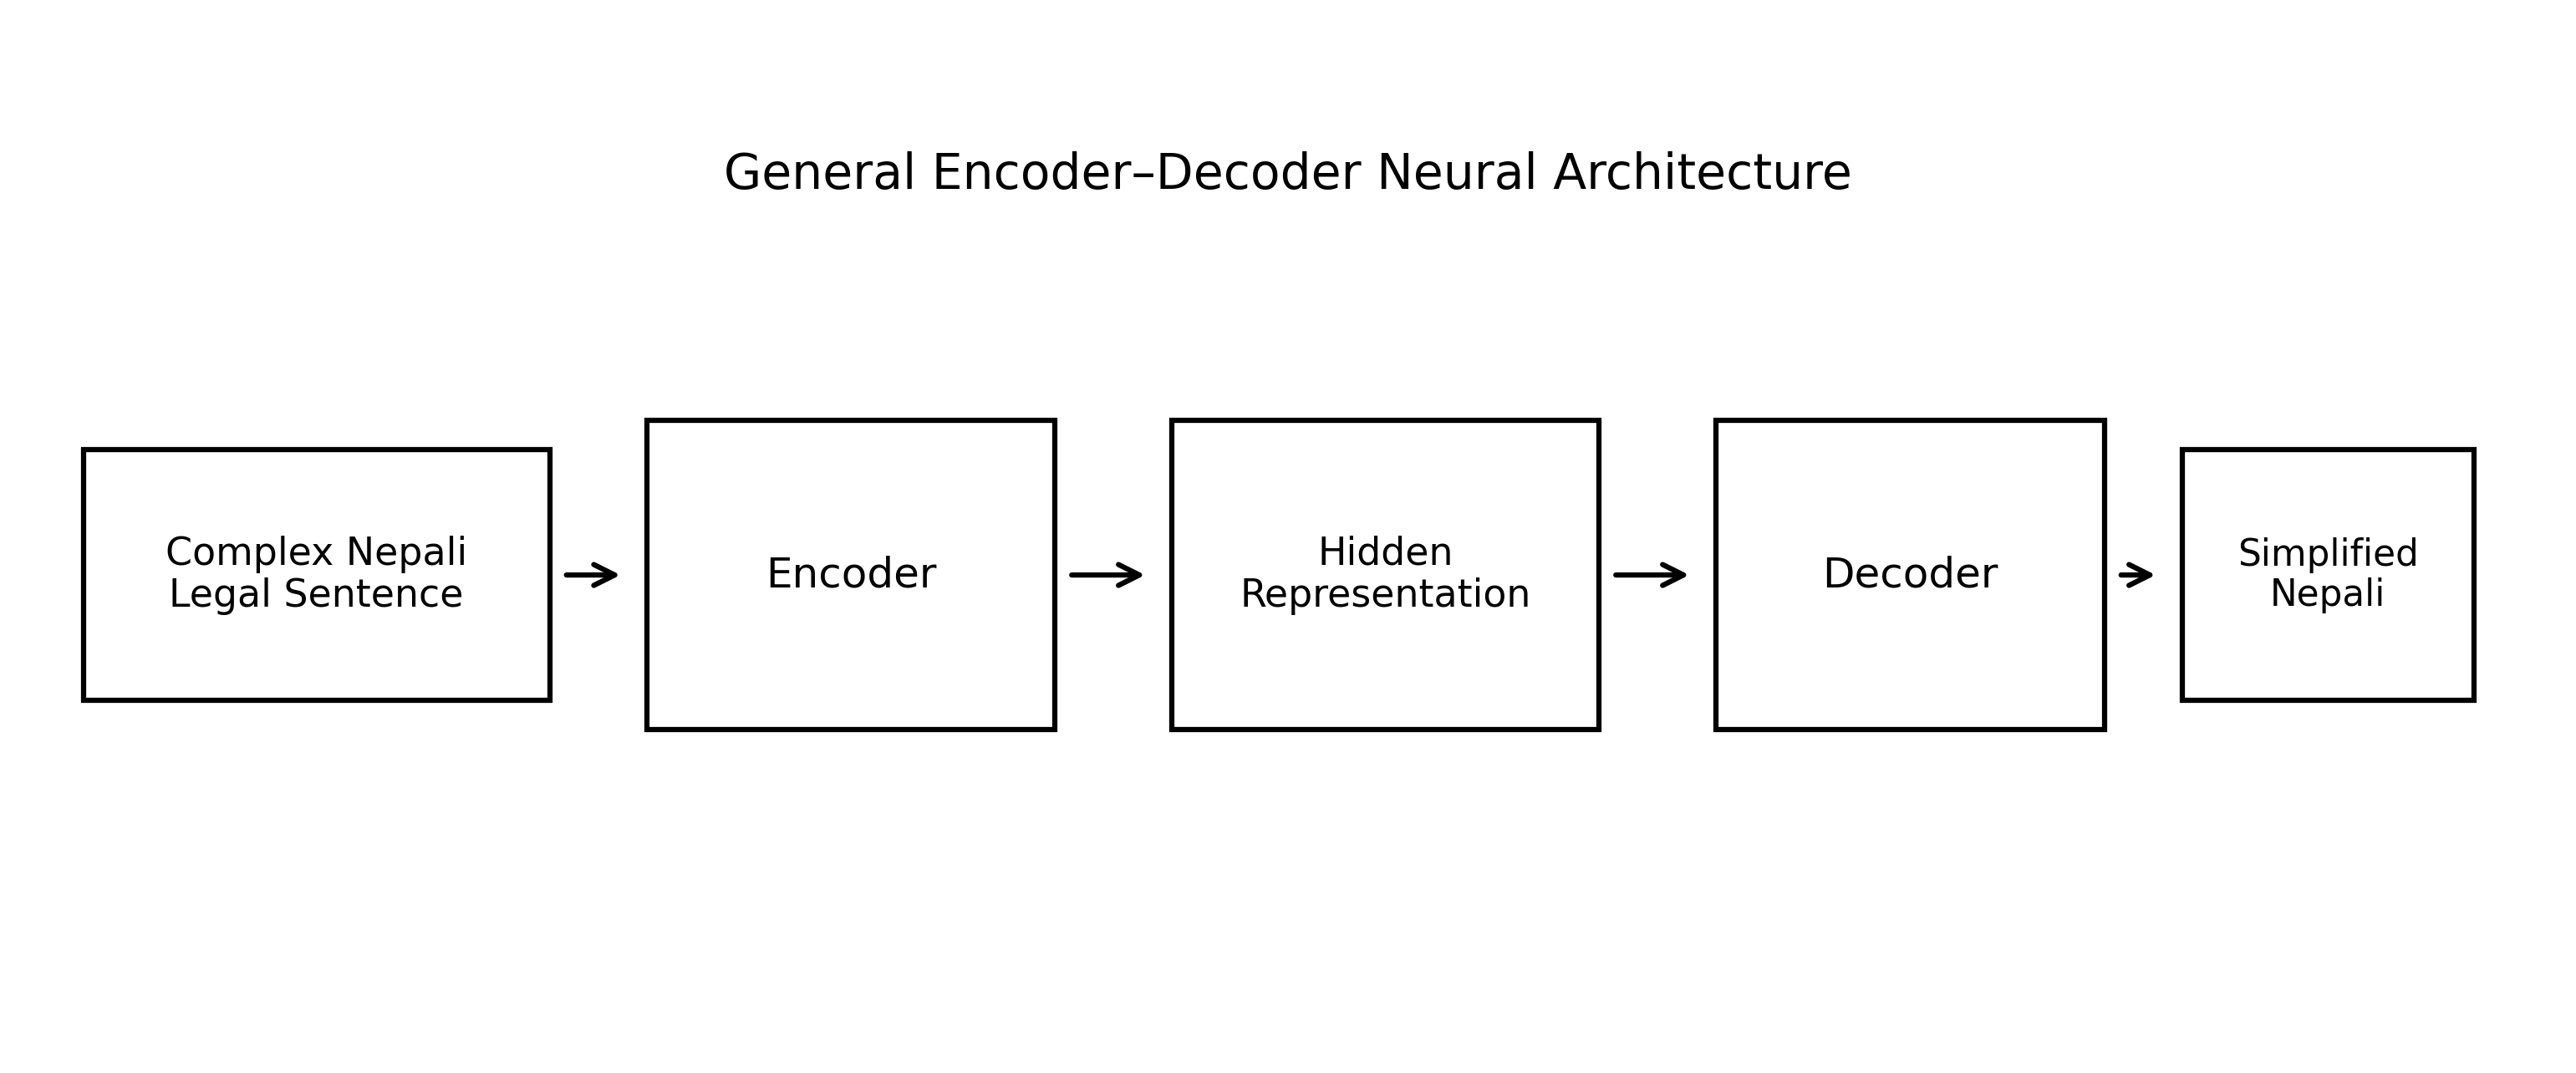
\includegraphics[width=0.88\textwidth]{seq2seq_neural_model_fixed.png}
    \caption{General encoder-decoder neural architecture for legal text simplification.}
    \label{fig:seq2seq_nn}
\end{figure}

\subsection{Transformer Architecture}

The Transformer architecture is the central model family used in this project. Unlike recurrent neural networks, the Transformer does not process tokens strictly one by one. Instead, it uses attention mechanisms to model relationships between all tokens in parallel. This is highly suitable for legal language, which often contains long clauses, nested conditions, and context-dependent meanings.

The Transformer consists of an encoder and a decoder. The encoder processes the input sentence and produces contextual hidden states, while the decoder generates the output sentence one token at a time. The theoretical breakthrough of the Transformer is the use of \textbf{self-attention}, which computes how strongly each token should attend to every other token in the sequence.

Given query matrix $Q$, key matrix $K$, and value matrix $V$, scaled dot-product attention is defined as:

\begin{equation}
\text{Attention}(Q,K,V) = \text{softmax}\left(\frac{QK^T}{\sqrt{d_k}}\right)V
\end{equation}

where $d_k$ is the dimension of the key vectors. The softmax term computes normalized importance weights, which determine how much information each token receives from the others.

To allow the model to capture several kinds of relationships at the same time, the Transformer uses \textbf{multi-head attention}. If there are $h$ attention heads, then:

\begin{equation}
\text{head}_i = \text{Attention}(QW_i^Q, KW_i^K, VW_i^V)
\end{equation}

\begin{equation}
\text{MultiHead}(Q,K,V) = \text{Concat}(\text{head}_1, \dots, \text{head}_h)W^O
\end{equation}

This allows different heads to focus on different aspects of the sentence, such as syntactic dependency, semantic similarity, clause boundaries, or condition markers.

After attention, the Transformer applies a position-wise feed-forward network:

\begin{equation}
\text{FFN}(x) = \max(0, xW_1 + b_1)W_2 + b_2
\end{equation}

Since the Transformer processes tokens in parallel, it also requires information about token order. This is handled using positional encodings. In the original Transformer, the positional encoding for position $pos$ and dimension $i$ is defined as:

\begin{equation}
PE(pos, 2i) = \sin\left(\frac{pos}{10000^{2i/d_{\text{model}}}}\right)
\end{equation}

\begin{equation}
PE(pos, 2i+1) = \cos\left(\frac{pos}{10000^{2i/d_{\text{model}}}}\right)
\end{equation}

These encodings allow the model to incorporate sequence order even though it does not use recurrence.

The model used in this project is \textbf{mT5}, which is a multilingual extension of the T5 architecture. T5 formulates all NLP tasks in a text-to-text manner. In this framework, a task is defined simply as input text mapped to output text. For legal simplification, the formulation is:

\begin{equation}
\text{Input: Complex Nepali legal sentence} \rightarrow \text{Output: Simplified Nepali sentence}
\end{equation}

This is particularly convenient because the same architecture can be used for simplification, paraphrasing, and explanation generation. mT5 extends this idea to 101 languages and thus provides a strong pretrained foundation for Nepali.

One challenge in multilingual generation is \textbf{accidental translation}, where the model may unexpectedly switch into a different language during generation. Since the target of this project must remain fully in Nepali, careful fine-tuning, task prompts, and decoding constraints are used to keep the output in the intended language and style.

In this project, the Transformer is used for \textbf{conditional generation}. It receives a complex Nepali legal sentence and produces a simpler Nepali sentence with the same meaning. This is more powerful than rule-based simplification because it can learn contextual rewrites such as:
\begin{itemize}
    \item replacing formal expressions with common words,
    \item splitting dense clauses into simpler form,
    \item preserving legal conditions and restrictions,
    \item simplifying syntax while retaining the legal force of the sentence.
\end{itemize}

However, the success of this approach still depends heavily on the quality of the training dataset. If the target simplifications remain too formal or vague, the model will learn weak simplification patterns. Therefore, model architecture and data quality must work together.

\begin{figure}[H]
    \centering
    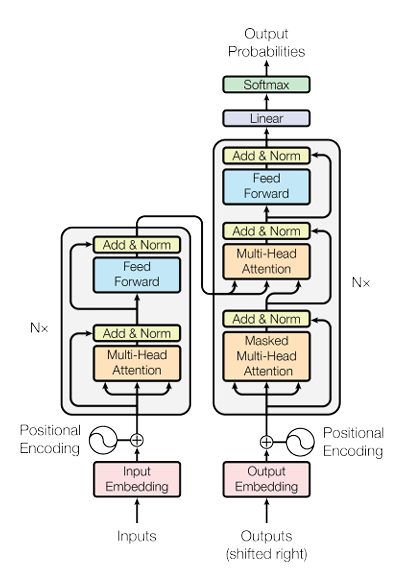
\includegraphics[width=0.88\textwidth]{Screenshot 2026-03-19 160014.png}
    \caption{Transformer encoder-decoder architecture used as the theoretical basis of the proposed simplification model.}
    \label{fig:transformer_architecture}
\end{figure}

\subsection{Text Preprocessing and Document Image Handling}

Although the core task of this project is text simplification, text preprocessing and document image handling form a crucial support pipeline. Legal materials are often obtained from PDF files, scanned documents, constitutional pages, or image-based legal archives. If the text is not machine-readable, it must first be extracted using optical character recognition.

Suppose an input image document is denoted by $I$. OCR can be viewed conceptually as a function:

\begin{equation}
T = f_{\text{OCR}}(I)
\end{equation}

where $T$ is the extracted text sequence. In practice, the quality of $T$ depends on image clarity, page layout, font style, scanning quality, and the OCR engine used. For legal text, OCR errors are highly problematic because even small distortions can change meaning, break sentence boundaries, or corrupt clause-level references.

The objective of document preprocessing is therefore to improve the quality of extracted text before dataset construction. Typical image-level preprocessing includes:
\begin{itemize}
    \item cropping margins and irrelevant borders,
    \item removing watermarks and page artifacts,
    \item improving contrast and readability,
    \item correcting skewed pages,
    \item reducing visual noise.
\end{itemize}

After OCR, text-level preprocessing is required. Let raw extracted text be denoted by $T_r$. The cleaned text $T_c$ is obtained by a normalization function:

\begin{equation}
T_c = g(T_r)
\end{equation}

where $g(\cdot)$ may include:
\begin{itemize}
    \item Unicode normalization,
    \item whitespace normalization,
    \item punctuation standardization,
    \item removal of duplicated symbols,
    \item correction of broken line joins,
    \item removal of headers, footers, and page numbers.
\end{itemize}

Once the text is cleaned, the next step is \textbf{segmentation}. Legal documents are usually long and cannot be used as single training examples. Therefore, each document is divided into smaller units such as sentences, clauses, or sub-clauses. If the cleaned text contains $N$ segments, it can be represented as:

\begin{equation}
T_c = \{s_1, s_2, s_3, \dots, s_N\}
\end{equation}

where each $s_i$ is a clause-level training candidate. Clause-level segmentation is particularly important in this project because legal meaning is often expressed compactly within one clause, and this helps keep the input within model limits while preserving semantic integrity.

After segmentation, each complex clause is manually rewritten into simpler Nepali. This is not ordinary paraphrasing. The simplified sentence must:
\begin{itemize}
    \item preserve the original legal meaning,
    \item avoid removing conditions or exceptions,
    \item replace overly formal words with simpler alternatives,
    \item use shorter and clearer sentence structure,
    \item avoid vague interpretation.
\end{itemize}

A dataset pair in this project therefore takes the form:

\begin{equation}
(s_i^{\text{complex}}, s_i^{\text{simple}})
\end{equation}

The overall dataset becomes:

\begin{equation}
D = \{(s_1^{\text{complex}}, s_1^{\text{simple}}), \dots, (s_n^{\text{complex}}, s_n^{\text{simple}})\}
\end{equation}

This dataset is finally stored in JSON or JSONL format using fields such as:
\begin{itemize}
    \item \texttt{complex\_nepali}
    \item \texttt{simplified\_nepali}
\end{itemize}

Thus, document image handling and preprocessing should be viewed as a \textbf{data quality pipeline}. In a low-resource project such as Nepali legal simplification, this pipeline is not secondary. It is one of the most important determinants of model quality because the performance of the Transformer depends directly on the correctness, cleanliness, and consistency of the training pairs.

\begin{figure}[H]
    \centering
    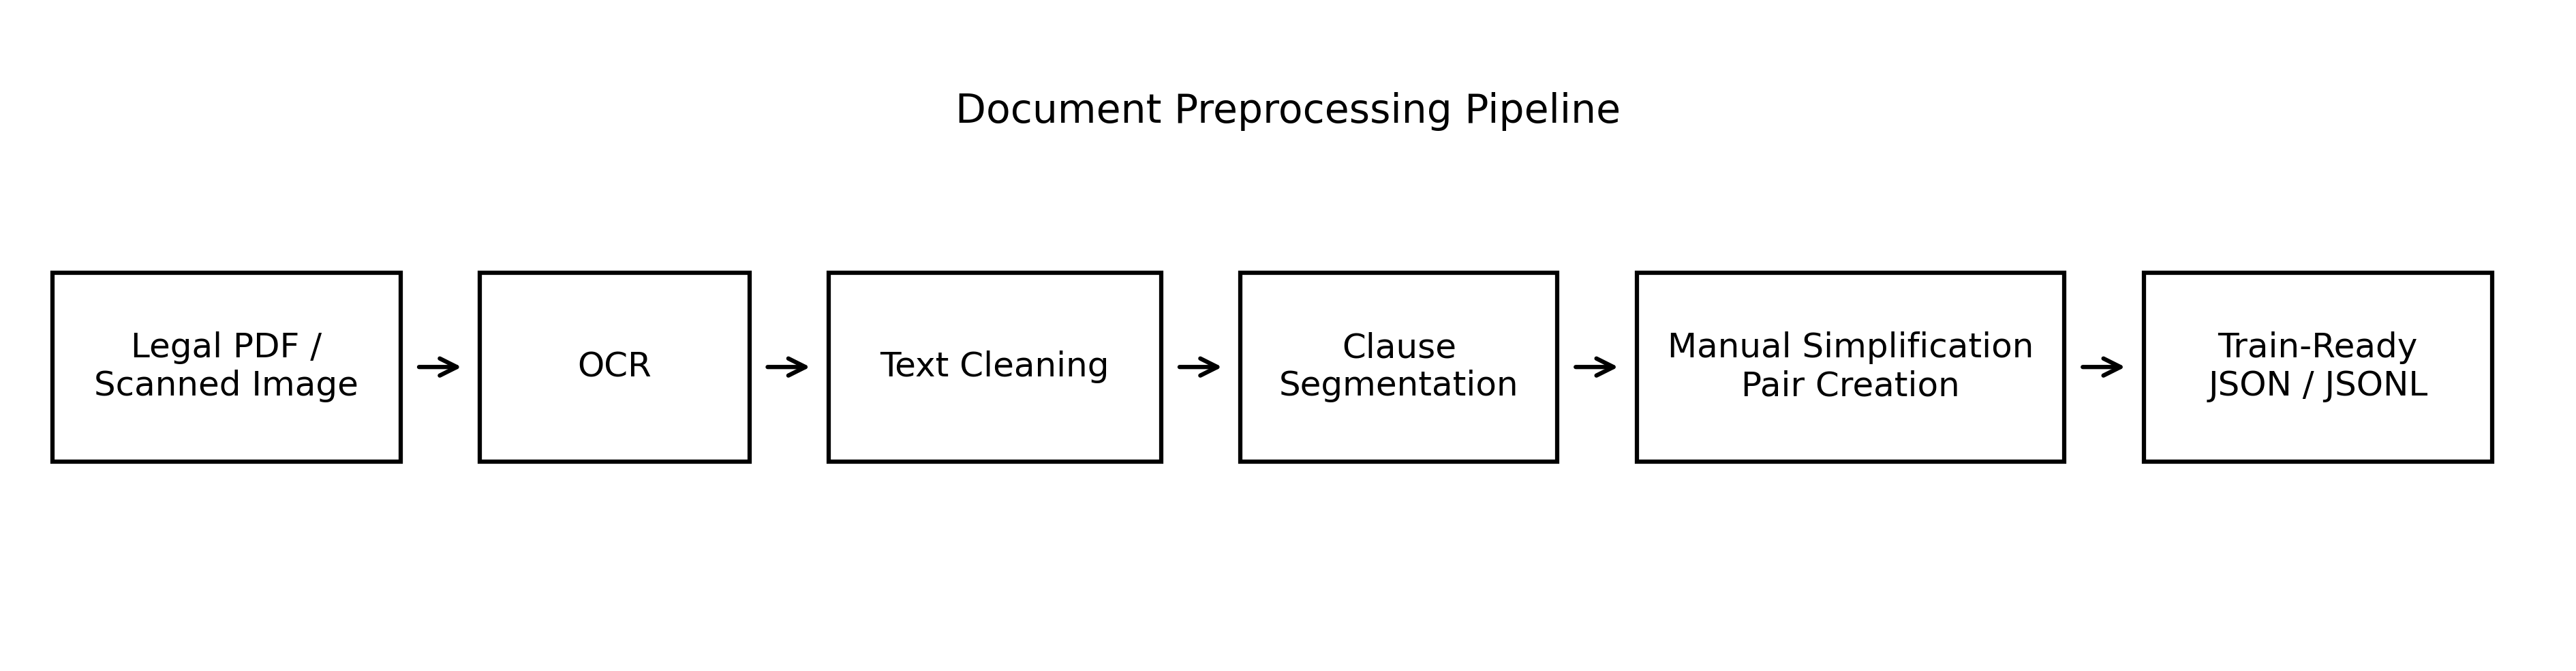
\includegraphics[width=0.95\textwidth]{preprocessing_pipeline.png}
    \caption{Document preprocessing pipeline: legal PDF/image, OCR, text cleaning, segmentation, simplification pair creation, and train-ready JSON dataset.}
    \label{fig:preprocessing_pipeline}
\end{figure}
\chapter{Methodology}

% \section{Methodology}

The methodology of this project is designed to develop a complete pipeline for simplifying complex Nepali legal and formal text into clearer and more understandable Nepali language. The overall process includes dataset preparation, model selection and fine-tuning, OCR-based text extraction, post-processing, and system development. In addition, the performance of the model is assessed through automatic evaluation metrics and human observation of generated outputs. The following subsections describe each stage of the methodology in detail.

\subsection{Data Curation and Pre-processing}

Data preparation is one of the most important stages of this project because the quality of the final simplified output depends heavily on the quality of the training data. For this project, a domain-specific Nepali simplification dataset was manually prepared from a variety of reliable and educationally relevant sources. These sources included selected legal and constitutional texts, as well as Nepali instructional and civic materials that contain formal language structures. The purpose of using such sources was to expose the model to complex sentence forms, legal terminology, and formal writing patterns commonly found in real-world Nepali documents.

The final dataset consists of \textbf{2,000 parallel sentence pairs}. Each pair contains an original complex Nepali sentence and its manually written simplified Nepali version. The dataset was prepared carefully so that the simplified sentence preserves the original meaning while making the language more accessible to general readers and students. Particular attention was given to preserving legal intent, restrictions, obligations, and conditions during simplification.

Each entry in the dataset includes the following fields:

\begin{itemize}
    \item \textbf{Original Nepali Text:} The complex sentence collected from the source document.
    \item \textbf{Simplified Nepali Text:} A manually simplified version of the original sentence written in clearer and more natural Nepali.
    \item \textbf{Vocabulary:} A list of difficult words or formal expressions from the source sentence along with their simpler Nepali meanings.
    % \item \textbf{English Translation:} An English translation of the simplified Nepali sentence for additional interpretability and multilingual support.
\end{itemize}

The data curation process involved manual sentence selection, sentence-level segmentation, simplification writing and vocabulary extraction. Long paragraphs and large constitutional or legal passages were first broken into smaller sentence-level or clause-level units so that each training example represented one central idea. This segmentation process was necessary because sequence-to-sequence models perform better when each input-output pair is concise, semantically aligned, and focused on a single meaning.

During simplification, emphasis was placed on the following principles:

\begin{itemize}
    \item preserving the original meaning of the sentence,
    \item reducing unnecessary legal or formal complexity,
    \item replacing difficult words with simpler alternatives where appropriate,
    \item maintaining grammatical correctness,
    \item avoiding distortion of rights, obligations, exceptions, and restrictions.
\end{itemize}

The dataset was also pre-processed before training. The pre-processing steps included Unicode normalization, whitespace cleanup, punctuation normalization, removal of duplicate entries, and correction of sentence boundary issues. Special care was taken to remove broken OCR-like fragments, incomplete expressions, and noisy text samples that could negatively affect training. Because Nepali text often contains irregular spacing and punctuation inconsistencies, normalization was necessary to make the dataset more uniform and model-friendly.

To maintain data quality, the prepared sentence pairs were manually reviewed. The simplified text was checked to ensure that it was shorter, clearer, and easier to understand than the source text, while still retaining the essential legal or formal meaning. Vocabulary entries were also reviewed so that the selected word explanations matched the context of the sentence.

The prepared corpus serves as the central training resource for the legal Nepali text simplification model.

\begin{figure}[H]
    \centering
    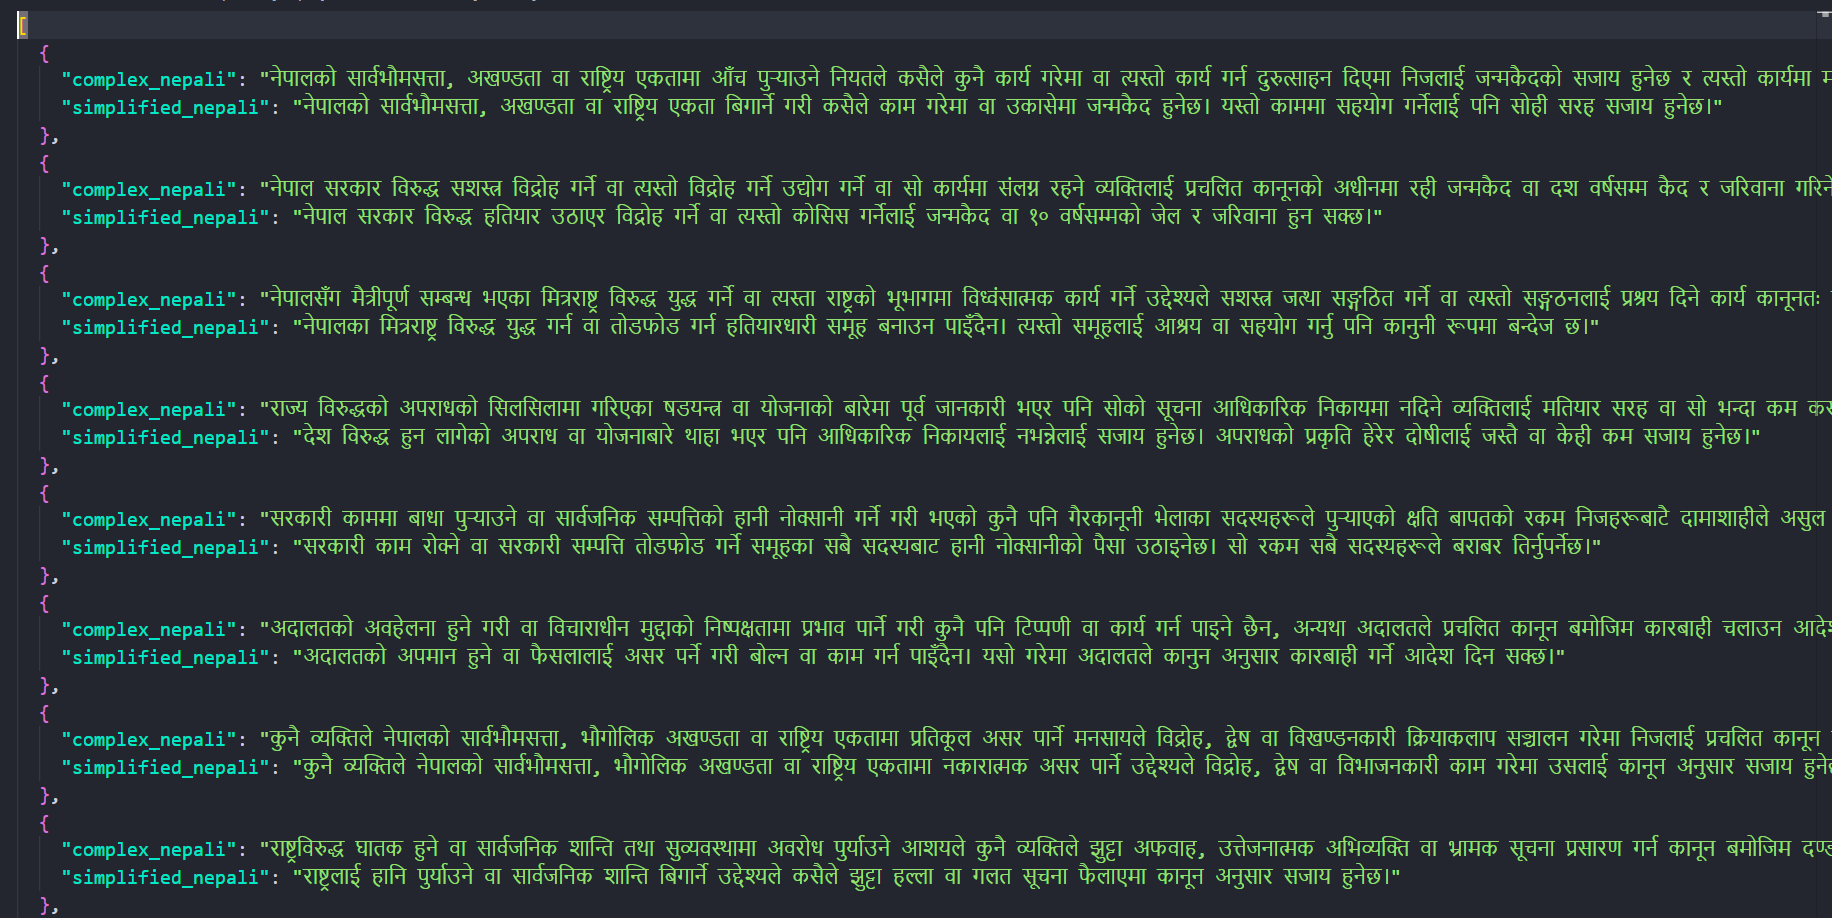
\includegraphics[width=0.8\textwidth]{Screenshot 2026-03-19 110620.png}
    \caption{Sample view of the curated Nepali simplification dataset}
    \label{fig:dataset1}
\end{figure}

% \begin{figure}[H]
%     \centering
%     \includegraphics[width=0.8\textwidth]{figures/dataset2.png}
%     \caption{Additional examples from the prepared dataset}
%     \label{fig:dataset2}
% \end{figure}

% \begin{figure}[H]
%     \centering
%     \includegraphics[width=0.8\textwidth]{.png}
%     \caption{Structure and contents of the final dataset}
%     \label{fig:dataset3}
% \end{figure}

\subsection{Model Selection and Fine-Tuning}

For the text simplification task, this project uses a Transformer-based sequence-to-sequence model. The selected architecture is \textbf{mT5}, which is a multilingual extension of the T5 model. This model is particularly suitable for the present work because it supports many languages, including Nepali, and is designed for text-to-text generation tasks. Since legal text simplification can be formulated as a mapping from complex text to simpler text, mT5 provides a natural modeling framework.

The model is fine-tuned rather than trained from scratch. Fine-tuning is preferred because pretrained multilingual models already contain broad linguistic knowledge learned from large corpora. This is especially important in low-resource language settings such as Nepali, where collecting massive domain-specific training data is difficult. By fine-tuning mT5 on the prepared legal simplification dataset, the model can adapt its general multilingual knowledge to the specific task of Nepali legal text rewriting.

The training process uses paired input-output samples. The original complex Nepali sentence is provided as the input, and the manually simplified Nepali sentence is used as the target output. During training, the model learns to generate a simplified sequence that is semantically aligned with the input while using simpler wording and structure.

The main training configuration includes the following components:

\begin{itemize}
    \item \textbf{Model:} mT5
    \item \textbf{Optimizer:} AdamW
    \item \textbf{Learning Rate:} 5e-5 (A conservative learning rate suitable for fine-tuning)
    \item \textbf{Batch Size:} 2  (Selected based on available GPU memory)
    \item \textbf{Epochs:} Multiple epochs with careful monitoring of validation performanc
    \item \textbf{Loss Function:} Cross-Entropy Loss
\end{itemize}

The input text is tokenized using the mT5 tokenizer, which is based on subword tokenization. This is especially effective for Nepali because it reduces out-of-vocabulary problems and handles morphologically rich words more efficiently than word-level tokenization. After tokenization, the source sequence is passed to the encoder, and the decoder learns to generate the simplified target sentence token by token.

To reduce the risk of overfitting, the training process follows a proper train-validation split. Validation loss is monitored throughout training to identify whether the model is learning meaningful simplification patterns or beginning to memorize the training samples. Since the dataset size is moderate, maintaining generalization is very important. Attention is also given to maximum source length and maximum target length so that the model does not truncate important content during training or generation.

The output generation settings are also important for this task. Since the model is multilingual, care is taken to ensure that the generated output remains in Nepali and does not switch to another language. Clean targets, consistent data formatting, and controlled generation settings help improve output quality and language consistency.

\subsection{OCR Integration and Post-processing}

In addition to direct text input, the system is designed to support legal or formal content extracted from image-based documents and scanned pages. For this purpose, an OCR pipeline is incorporated into the methodology. This allows the system to accept document images and convert them into machine-readable Nepali text before simplification.

The OCR component is based on \textbf{Tesseract OCR} with Nepali language support. Tesseract is selected because it is open-source, widely used, and capable of extracting printed text from image documents. However, raw OCR output is often noisy, especially when the source image contains skew, blur, low contrast, page artifacts, or irregular formatting. Therefore, OCR is not treated as a single-step extraction process but as part of a broader preprocessing pipeline.

Before OCR is applied, the document image undergoes basic image preprocessing. These preprocessing operations may include:

\begin{itemize}
    \item noise reduction,
    \item contrast enhancement,
    \item image sharpening,
    \item margin cropping,
    \item binarization,
    \item alignment correction.
\end{itemize}

These steps improve the readability of the image and increase the accuracy of text extraction. Once the OCR text is extracted, post-processing is applied to refine the output. This includes correction of spacing errors, normalization of punctuation, removal of broken line artifacts, and correction of common OCR mistakes in Nepali characters. If necessary, a custom Nepali word list or dictionary can be used to identify and correct invalid or suspicious tokens.

The OCR text is then segmented into usable sentence units before being passed to the simplification model. This segmentation is important because raw OCR often produces paragraph-like blocks or line-fragmented text that are not directly suitable as model input. By converting the raw OCR output into cleaner sentence-level units, the overall simplification pipeline becomes more reliable and effective.

\subsection{System Architecture and Development}

The complete system is designed as a web-based application so that users can easily interact with the simplification model through a user-friendly interface. The system follows a modular architecture consisting of a backend processing layer and a frontend interaction layer.

The \textbf{backend} is responsible for handling text input, OCR processing, model inference, and result generation. A lightweight and efficient API framework such as FastAPI can be used to serve the trained model and manage processing requests. The backend receives the raw user input, applies the necessary preprocessing steps, runs the simplification model, and returns the generated output in a structured form.

The \textbf{frontend} provides the user interface through which users can enter text or upload files. A modern frontend framework can be used to create an interactive and responsive environment. The user interface is designed to support the following functions:

\begin{itemize}
    \item direct text input for legal or formal Nepali sentences,
    \item image or document upload for OCR-based extraction,
    \item display of simplified Nepali output,
    \item display of difficult-word vocabulary with simple meanings,
    % \item display of English translation where needed,
    \item organized layout for easy readability.
\end{itemize}

The overall architecture supports a practical workflow in which users submit complex text, the system processes the content, and the final simplified result is returned in a clear format. This design makes the project suitable not only as a research prototype but also as a potentially useful educational and assistive tool.

\subsection{Evaluation Strategy}

The performance of the simplification model is evaluated using both automatic metrics and manual observation. Since legal and formal text simplification requires preservation of meaning as well as readability improvement, evaluation must consider both textual similarity and output quality.

For quantitative evaluation, two standard metrics are used:

\begin{itemize}
    \item \textbf{BLEU}
    \item \textbf{ROUGE-L}
\end{itemize}

BLEU is used to measure the overlap between the generated simplified sentence and the reference simplified sentence. It provides an indication of how closely the model output matches the expected wording. ROUGE-L is used to measure sequence-level similarity based on the longest common subsequence, which is useful for text generation tasks where exact token matching may vary but structural similarity still matters.

These two metrics provide a basic numerical indication of model performance on the test set. However, automatic metrics alone are not sufficient for legal simplification because a sentence may have acceptable metric values while still containing awkward phrasing, incomplete simplification, or slight meaning distortion.

For this reason, \textbf{human eye evaluation} is also performed. The generated outputs are manually inspected to check whether:

\begin{itemize}
    \item the simplified sentence preserves the original meaning,
    \item the wording is easier to understand,
    \item the sentence remains grammatically correct,
    \item key legal conditions, restrictions, and obligations are retained,
    \item the output remains fully in Nepali and does not contain irrelevant or broken text.
\end{itemize}

Manual observation is particularly important in this project because simplification quality is not determined only by textual similarity. A good output must also be clear, natural, and semantically faithful. Therefore, the final evaluation combines metric-based analysis with human judgment of output quality.

\subsection{Overall Workflow}

The complete methodology of the project can be summarized as a sequential workflow:

\begin{enumerate}
    \item Collect complex Nepali legal and formal sentences from relevant documents.
    \item Prepare simplified Nepali versions and vocabulary mappings
    \item Clean and normalize the dataset for model training.
    \item Fine-tune the mT5 model on the parallel simplification dataset.
    \item Extract text from document images using OCR when required.
    \item Apply preprocessing and post-processing to improve extracted text quality.
    \item Pass the clean text to the simplification model.
    \item Generate simplified Nepali output.
    \item Evaluate the output using BLEU, ROUGE-L, and human observation.
\end{enumerate}

This methodology provides a complete framework for developing a Nepali legal text simplification system that is both technically sound and practically useful.
---

\chapter{ Experimental Setup}


\subsection*{Model Architecture}
A Transformer-based model, \textbf{mT5-base}, was fine-tuned for text-to-text generation tasks.

\subsection*{Dataset}
A custom-curated parallel corpus of 5,000 sentence pairs covering Nepali civic and legal texts was used. The dataset was stored and managed in \texttt{CSV} format. However, for the technical implementation of model training, it is converted to \texttt{JSON}.

\subsection*{Hardware}
Training was conducted on a GPU-enabled system (e.g., \textbf{NVIDIA T4} or \textbf{V100}) using Google Colab.

\subsection*{Software and Frameworks}
\begin{itemize}
    \item \textbf{Backend:} Python 3.9+, PyTorch, Hugging Face Transformers, FastAPI
    \item \textbf{Frontend:} React.js
    \item \textbf{OCR:} Tesseract OCR with Nepali language pack
\end{itemize}

\subsection*{Key Hyperparameters}
\begin{itemize}
    \item \textbf{Optimizer:} AdamW
    \item \textbf{Learning Rate:} 5e-5
    \item \textbf{Batch Size:} 2  (Selected based on available GPU memory)
    \item \textbf{Epochs:} 15 (without early stopping)
\end{itemize}

\subsection*{Evaluation Metrics}
\begin{itemize}
    \item \textbf{Quantitative:} BLEU and ROUGE-L scores
    \item \textbf{Qualitative:} Human evaluation and end-users
\end{itemize}



\chapter{Proposed System Design}
% \begin{figure}[h]
%     \centering
%     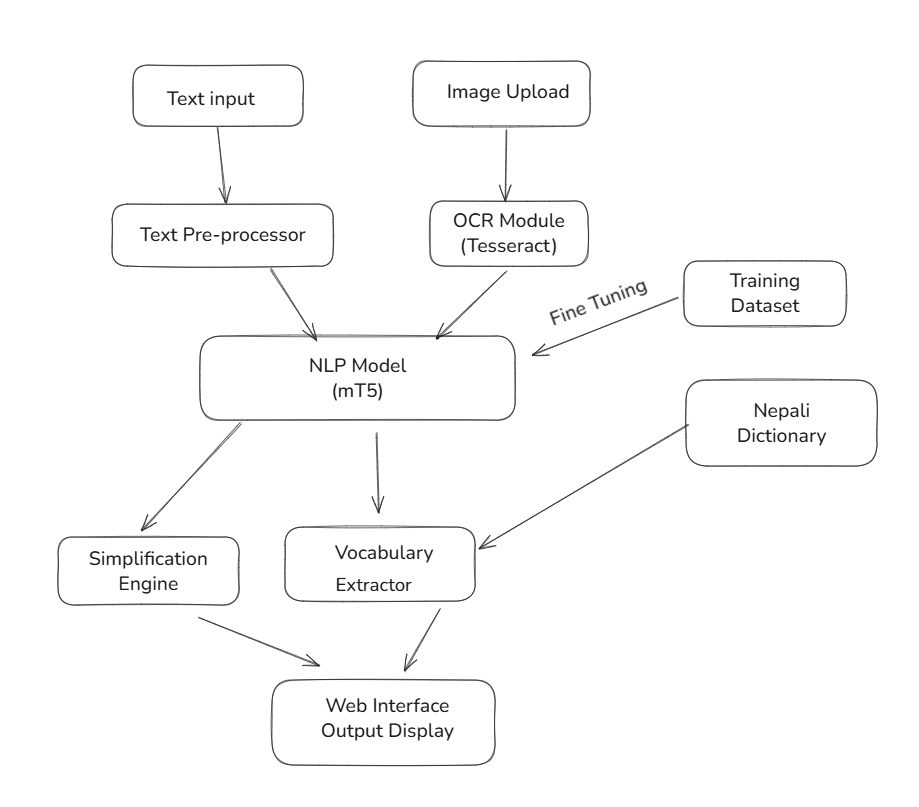
\includegraphics[width=0.9\textwidth]{System Design.png}
%     \caption{System Architecture of the model}
%     \label{fig:System Architecture}
% \end{figure}

\section{System Architecture and Technical Implementation}

This section describes the architecture and technical implementation of the proposed Nepali Text Simplification System. The system is designed in a modular manner so that input handling, preprocessing, model inference, vocabulary extraction, and output presentation are organized into separate but connected stages. Such a modular design improves system clarity, maintainability, and future extensibility. The overall architecture of the system is illustrated in Figure~\ref{fig:system_architecture}.

\begin{figure}[H]
    \centering
    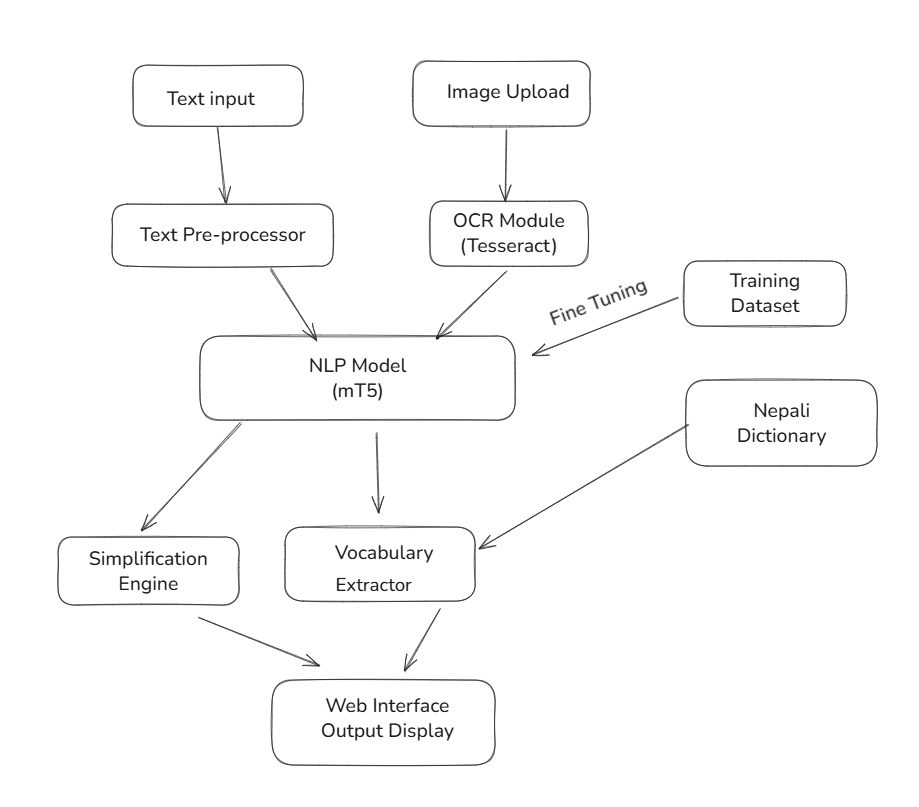
\includegraphics[width=0.9\textwidth]{System Design.png}
    \caption{System architecture of the proposed Nepali text simplification system}
    \label{fig:system_architecture}
\end{figure}

The system accepts user input in two forms: direct text input and image upload. The entered or extracted text is then processed through a preprocessing layer and passed to the central NLP model based on mT5. The model performs the simplification task, while a separate vocabulary extraction component identifies difficult words and their simpler meanings using a Nepali dictionary. Finally, the processed outputs are displayed through the web interface.

\subsection{Input Layer}

The input layer serves as the entry point of the system. It allows users to provide content either by typing Nepali text directly into the application or by uploading an image containing Nepali text. This dual-input design increases the practical usability of the system, as users may have either machine-readable text or scanned/image-based legal documents.

\subsubsection{Text Input}

The text input component is intended for users who already have the source Nepali text in editable form. On the frontend, this is implemented using a standard HTML \texttt{textarea} element. The user types or pastes the legal or formal Nepali sentence into this input area and then submits it for processing.

From the implementation perspective, when the user clicks the action button, the frontend JavaScript captures the input text and sends it to the backend server through an HTTP POST request. This is commonly handled using the \texttt{fetch()} API. The text is transmitted as a string payload and received by the backend for further preprocessing. This path is efficient because it avoids OCR and directly forwards machine-readable text into the simplification pipeline.

\subsubsection{Image Upload}

The image upload component supports cases where the source text is available only in image format, such as scanned legal documents, screenshots, or photographed pages. On the frontend, this functionality is implemented using an HTML file input element such as \texttt{<input type="file">}. The user can upload image files such as JPG or PNG, and in extended implementations PDF pages may also be supported.

After the file is selected, the frontend submits it to the backend as \texttt{multipart/form-data}. The backend temporarily stores the uploaded file and forwards it to the OCR module. This path is especially useful for document digitization and broadens the accessibility of the system beyond plain text input.

\subsection{Pre-processing Layer}

The preprocessing layer converts raw user input into a cleaner and more standardized text form before it is given to the NLP model. Since model performance depends strongly on input quality, this stage plays an essential role in improving the reliability of the overall system.

\subsubsection{Text Pre-processor}

The text pre-processor handles the raw text obtained from the text input path. This module is implemented in Python and performs several normalization and cleaning operations. These operations include removing unnecessary whitespace, correcting inconsistent punctuation, handling Unicode normalization for Devanagari script, and resolving common text formatting issues.

In addition, the text pre-processor may split long text into sentence-level units if necessary. This is especially important when dealing with legal or formal Nepali documents, where long paragraphs may contain several clauses or multiple sentences. Standard Python string operations and the \texttt{re} library for regular expressions can be used for these tasks.

The output of this module is a clean text sequence that is more suitable for tokenization and inference by the mT5 model.

\subsubsection{OCR Module (Tesseract)}

The OCR module handles the input received from the image upload path. Its main function is to extract machine-readable Nepali text from the uploaded image. This module is based on Tesseract OCR, which is integrated through the Python wrapper \texttt{pytesseract}.

Before passing the image to Tesseract, the backend may apply basic image preprocessing steps using libraries such as Pillow or OpenCV. These steps may include grayscale conversion, noise reduction, contrast enhancement, thresholding, or image sharpening. Such operations improve OCR quality by making the text more visually distinct from the background.

Tesseract is configured with the Nepali language pack so that it can recognize Devanagari script more accurately. After OCR processing, the extracted text is returned as a raw string. Since OCR output may contain broken words, spacing issues, or character-level mistakes, the extracted text may also pass through additional normalization before being sent to the NLP model.

\subsection{Core Processing Layer: NLP Model (mT5)}

The central component of the system is the NLP model, which performs the main text simplification task. This project uses mT5, a multilingual Transformer-based encoder-decoder model designed for text-to-text generation tasks. The choice of mT5 is appropriate because it supports Nepali and is capable of learning contextual rewriting patterns through fine-tuning.

\subsubsection{NLP Model (mT5)}

The mT5 model is loaded on the backend using the Hugging Face \texttt{transformers} library. It receives the cleaned Nepali input text, tokenizes it into subword units, processes the sequence through its encoder-decoder architecture, and generates a simplified Nepali output sequence.

Since the model is based on the Transformer architecture, it can capture long-range dependencies and contextual relationships in legal or formal sentences. This is especially useful for Nepali legal simplification, where the meaning of a sentence often depends on condition markers, exception clauses, or formal legal expressions.

\subsubsection{Fine-Tuning with Training Dataset}

The model is specialized for the simplification task through a fine-tuning process on the prepared Nepali dataset. This dataset contains parallel examples of complex Nepali sentences and their manually simplified Nepali versions. The training dataset is used in an offline stage to adapt the pretrained mT5 model to the domain of legal and formal Nepali simplification.

During training, the original Nepali sentence is used as the input sequence and the simplified Nepali sentence is used as the target sequence. The model learns to minimize generation loss and gradually becomes better at rewriting complex input text into simpler and clearer Nepali language.

The fine-tuned model weights are then saved and loaded into the deployed system. In the live application, the backend does not retrain the model; it only performs inference using the already fine-tuned model.

\subsection{Output Generation Layer}

Once the central NLP model processes the text, the system generates outputs through two main components: the simplification engine and the vocabulary extractor. These modules work together to provide both a simplified sentence and lexical support for difficult words.

\subsubsection{Simplification Engine}

The simplification engine is the functional use of the fine-tuned mT5 model for generating simplified Nepali text. It is not a separate standalone model outside the architecture, but rather the operational stage in which the model's \texttt{generate()} method is called on the cleaned input.

The model produces a simplified output sequence by decoding token predictions step by step. This output is designed to preserve the meaning of the original sentence while making the wording more understandable for general readers or students. The simplification engine therefore forms the main result-producing component of the system.

\subsubsection{Vocabulary Extractor}

The vocabulary extractor is a rule-based module that works alongside the simplification engine. Its purpose is to identify difficult or formal Nepali words from the original input and provide their simpler meanings. This improves user understanding and adds educational value to the system.

Technically, this module uses a Nepali dictionary implemented as a Python dictionary or hash map. The dictionary stores mappings between difficult words and their simpler Nepali explanations. During execution, the original input text is tokenized into words, and each token is checked against the stored dictionary entries. If a match is found, the corresponding simpler meaning is retrieved and added to the vocabulary output.

This design is lightweight and efficient, and it complements the neural simplification output by giving users direct word-level assistance.

\subsection{Presentation Layer}

The presentation layer is responsible for displaying the final outputs to the user through the web interface. After simplification and vocabulary extraction are completed, the backend combines the outputs into a structured response format, typically JSON.

The frontend receives this response and dynamically updates the web page to display the generated results. Separate sections of the interface can be used to show the simplified Nepali text and the extracted vocabulary meanings in an organized way. This makes the system easy to use and improves readability of the generated content.

The web interface acts as the final interaction point between the system and the user. It hides the internal technical complexity of OCR, preprocessing, and model inference, and instead presents the output in a simple and accessible manner.

\subsection{Overall System Flow}

The complete technical flow of the system can be summarized as follows:

\begin{enumerate}
    \item The user provides input either through direct text entry or image upload.
    \item If the input is text, it is sent to the text pre-processor.
    \item If the input is an image, it is sent to the OCR module for text extraction.
    \item The cleaned text is forwarded to the fine-tuned mT5 model.
    \item The model generates simplified Nepali text.
    \item The vocabulary extractor identifies difficult words and retrieves their simpler meanings from the Nepali dictionary.
    \item The simplification output and vocabulary output are sent to the frontend.
    \item The web interface displays the final results to the user.
\end{enumerate}

Thus, the proposed architecture combines OCR, text preprocessing, Transformer-based simplification, and dictionary-based vocabulary support into a unified web-based system for Nepali text simplification.

\chapter{Results and Discussion}
% \addcontentsline{toc}{chapter}{\numberline{}Results and Discussion}


For evaluating the proposed \textbf{SajiloText} system based on the \textbf{mT5} model, the performance of the trained model was analyzed using both \textbf{BLEU} and \textbf{ROUGE} metrics on the validation set. In addition to the final text generation quality, the behavior of the model during training was also examined through the \textbf{training loss} and \textbf{validation loss} curves. These results help assess not only how well the model learns the simplification task, but also how effectively it generalizes to unseen Nepali legal text.

\section{Model Evaluation}

The individual BLEU and ROUGE results obtained during model training and validation are presented below.

\subsection{BLEU Score Analysis}

The BLEU score was used as the primary model selection metric because it provides a quantitative measure of overlap between the generated simplified sentence and the reference simplified sentence. Figure~6.1 presents the BLEU score progression across epochs together with the corresponding training and validation loss curves.

It can be observed that the model improves rapidly during the initial epochs. The BLEU score increases from 33.63 in the first epoch to 72.80 by the fourth epoch, showing that the model quickly learns the mapping between complex legal Nepali text and its simplified form. After this stage, the BLEU score continues to improve gradually and reaches its highest value of 77.81 at epoch 19. This indicates that the model achieves its best generation quality at that checkpoint.

At the same time, the training loss decreases steadily from 11.7748 in epoch 1 to 0.3783 in epoch 20, which confirms that the model is learning the training distribution effectively. The validation loss also decreases significantly during the early epochs and then stabilizes around 0.80 -- 0.84. This behavior suggests that the model converges properly and does not suffer from severe overfitting. Although the training loss continues to decrease after epoch 10, the validation loss remains nearly constant, which indicates mild saturation in learning. Therefore, selecting the model from epoch 19 based on the highest BLEU score is a reasonable choice.
\begin{figure}[H]
    \centering
    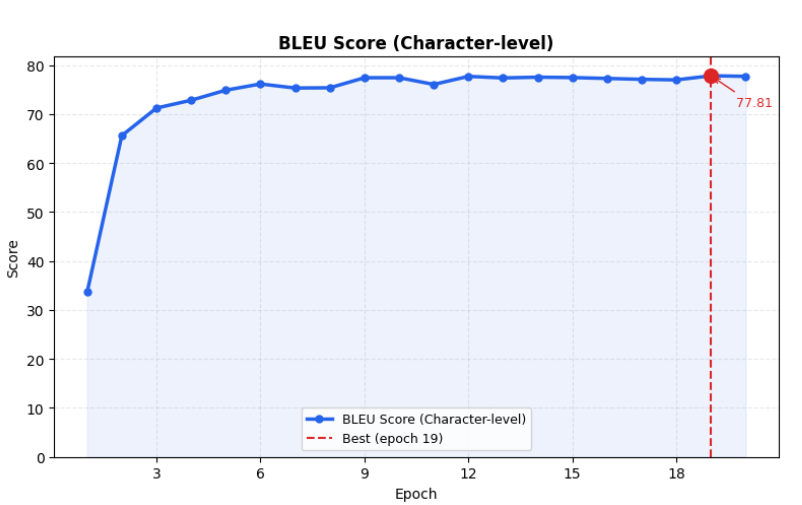
\includegraphics[width=\textwidth]{Bleuscore.png}
    \caption{BLEU score per epoch and training versus validation loss for the SajiloText mT5 model. The best checkpoint is obtained at epoch 19 with a BLEU score of 77.81.}
    \label{fig:bleu_results}
\end{figure}
\begin{figure}[H]
    \centering
    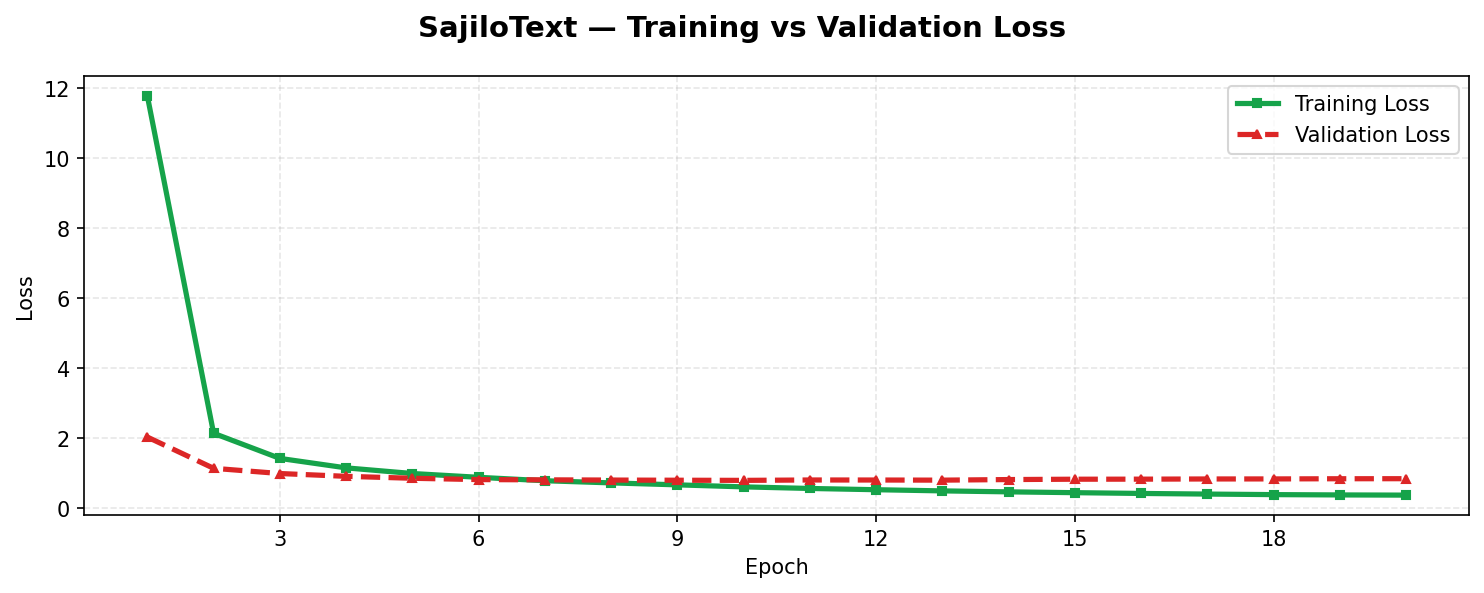
\includegraphics[width=\textwidth]{loss_curves.png}
    \caption{Training vs Validation Loss Graph}
    \label{fig:trainval_loss_results}
\end{figure}

The detailed epoch-wise training summary is presented in Table~\ref{tab:training_summary}. The table shows that the model maintains a consistent improvement trend throughout the training process. Even after the best epoch is reached, the BLEU score remains stable, demonstrating that the model performance is robust across later epochs.

\begin{table}[H]
\centering
\caption{Epoch-wise training summary of the SajiloText mT5 model}
\label{tab:training_summary}
\small
\begin{tabular}{cccc}
\toprule
\textbf{Epoch} & \textbf{Train Loss} & \textbf{Validation Loss} & \textbf{BLEU Score} \\
\midrule
1  & 11.7748 & 2.0357 & 33.63 \\
2  & 2.1442  & 1.1438 & 65.58 \\
3  & 1.4268  & 0.9949 & 71.21 \\
4  & 1.1564  & 0.9151 & 72.80 \\
5  & 0.9954  & 0.8594 & 74.86 \\
6  & 0.8870  & 0.8218 & 76.13 \\
7  & 0.7889  & 0.8148 & 75.30 \\
8  & 0.7276  & 0.8083 & 75.35 \\
9  & 0.6717  & 0.8035 & 77.40 \\
10 & 0.6139  & 0.7995 & 77.41 \\
11 & 0.5685  & 0.8106 & 76.04 \\
12 & 0.5327  & 0.8095 & 77.68 \\
13 & 0.4993  & 0.8060 & 77.36 \\
14 & 0.4718  & 0.8227 & 77.52 \\
15 & 0.4483  & 0.8326 & 77.43 \\
16 & 0.4262  & 0.8343 & 77.26 \\
17 & 0.4083  & 0.8395 & 77.08 \\
18 & 0.3929  & 0.8408 & 76.96 \\
\text{19} &\text {0.3838}  & \textbf {0.8462} & \textbf {77.81} \\
20 & 0.3783  & 0.8474 & 77.68 \\
\bottomrule
\end{tabular}
\end{table}

From Table~\ref{tab:training_summary}, it is clear that the model reaches its best validation generation quality at epoch 19. While the training loss continues to decrease slightly afterwards, the BLEU score does not improve further in a significant way. This further supports the use of epoch 19 as the final model checkpoint for text simplification.

\subsection{ROUGE Score Analysis}

In addition to BLEU, the generated simplified outputs were also evaluated using ROUGE-1, ROUGE-2, and ROUGE-L scores at the Nepali word level on the full validation set. These metrics measure unigram overlap, bigram overlap, and sequence-level similarity between the generated output and the reference simplification.

The epoch-wise progression of ROUGE scores is illustrated in Figures~6.2, 6.3, and 6.4. It can be observed that all three ROUGE metrics improve rapidly during the early stages of training and gradually stabilize after later epochs, indicating proper convergence of the model.

The ROUGE-1 F1 score increases significantly from 0.3151 in epoch 1 to 0.6804 by epoch 3, eventually reaching its highest value of 0.7727 at epoch 19. This demonstrates that the model effectively preserves the major lexical content of the reference simplified sentences.

Similarly, the ROUGE-2 F1 score improves from 0.1540 in the first epoch to 0.5113 by epoch 3 and achieves its best value of 0.6609 at epoch 19. Since ROUGE-2 evaluates bigram overlap, this result indicates that the model can generate meaningful local word sequences and maintain phrase-level consistency in simplified Nepali legal text.

The ROUGE-L F1 score also shows a stable improvement trend throughout training. Starting from 0.3046 in epoch 1, the score rises steadily and reaches its maximum value of 0.7628 at epoch 19. ROUGE-L measures the longest common subsequence similarity, and the high value suggests that the generated outputs preserve overall sentence structure and semantic flow effectively.

\begin{table}[H]
\centering
\caption{ROUGE evaluation results on the full validation set}
\label{tab:rouge_results}
\small
\begin{tabular}{ccccc}
\toprule
\textbf{Metric} & \textbf{F1 Score} & \textbf{Percentage} & \textbf{Target} \\
\midrule
ROUGE-1 & 0.7727 & 77.27\% & $> 0.50$   \\
ROUGE-2 & 0.6609 & 66.09\% & $> 0.30$   \\
ROUGE-L & 0.7628 & 76.28\% & $> 0.45$ \\
\bottomrule
\end{tabular}
\end{table}

All three ROUGE scores reach high values and remain stable during the later epochs, which confirms that the model performs consistently well on the text simplification task. The relatively high ROUGE-1 and ROUGE-L values indicate that the generated outputs successfully preserve the main meaning and overall sentence flow of the original text, while the strong ROUGE-2 score demonstrates that phrase-level accuracy is also maintained.

The training curves further show that the ROUGE metrics begin to saturate after approximately epoch 10, even though the training loss continues to decrease slightly. This suggests that the model has already learned most of the important lexical and structural simplification patterns by that stage. The best checkpoint is obtained at epoch 19, where all ROUGE metrics achieve their highest values simultaneously.\\
Figures~6.3, and 6.4 illustrate the epoch-wise progression of ROUGE-1, ROUGE-2, and ROUGE-L scores, respectively. The epoch-wise ROUGE curves shown in Figures~ 6.3, and 6.4 demonstrate a rapid improvement during the early training stages followed by gradual stabilization in later epochs. The highlighted peak points in the curves correspond to the best-performing checkpoint at epoch 19, where the model achieves the highest ROUGE-1, ROUGE-2, and ROUGE-L scores. The smooth and stable behavior of the curves after convergence indicates that the proposed mT5-based SajiloText model is capable of generating simplified Nepali legal text with strong lexical overlap, phrase consistency, and structural preservation.

\begin{figure}[H]
    \centering
    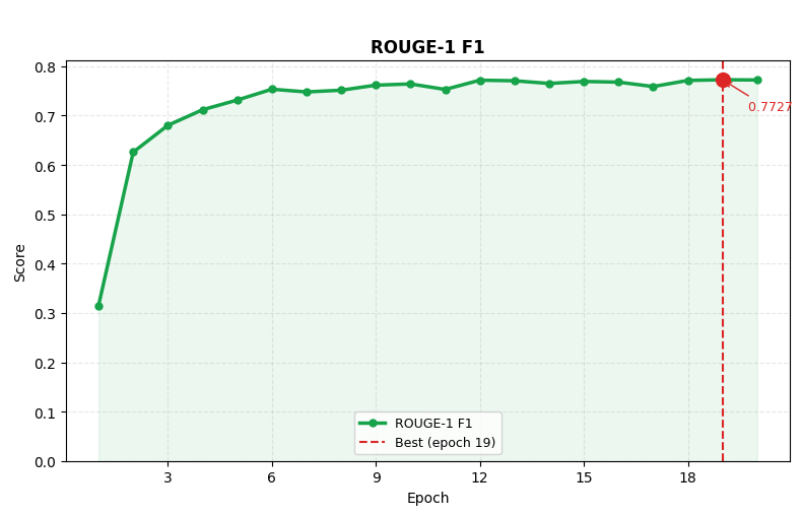
\includegraphics[width=\textwidth]{Ro1.png}
    \caption{Distribution of ROUGE-1}
    \label{fig:rouge_distribution}
\end{figure}

\begin{figure}[H]
    \centering
    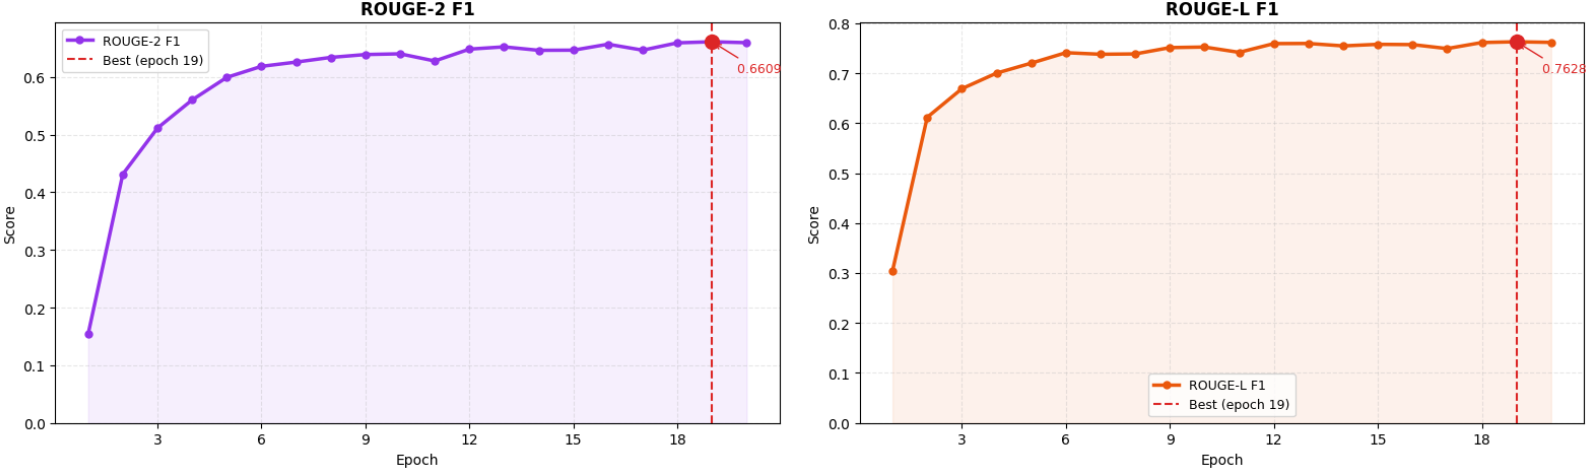
\includegraphics[width=\textwidth]{Ro2.png}
    \caption{Distribution of ROUGE-2  and ROUGE-L scores}
    \label{fig:rouge_distribution}
\end{figure}

\subsection{SARI Score Analysis}

The SARI (System output Against References and against the Input) score is a 
standard automatic evaluation metric specifically designed for text simplification 
tasks, making it particularly relevant to the SajiloText project. Unlike BLEU and 
ROUGE, which measure similarity between a system output and a reference text, SARI 
evaluates three distinct simplification operations simultaneously: the addition of 
new words not present in the source, the retention of words that should be kept 
from the source, and the deletion of complex words that should be removed. Each 
operation is scored using n-gram precision and recall across 1 to 4-gram levels, 
and the final SARI score is computed as the arithmetic mean of these three component 
scores, expressed on a scale of 0 to 100.

For the SajiloText system, SARI was computed after every training epoch using a 
custom implementation built from scratch using Nepali-aware whitespace tokenization. 
This was necessary because standard SARI libraries such as \texttt{sacrebleu} and 
\texttt{easse} rely on regex-based tokenization that strips Devanagari Unicode 
characters, producing zero scores for Nepali text. The custom implementation 
correctly handles Nepali morphology by splitting on whitespace and stripping dandas 
(\devanagarifont{।}) and common punctuation before n-gram computation.

SARI scores were computed on the validation set of 145 pairs after each of the 20 
training epochs. A SARI score above 40 is generally considered good for text 
simplification systems, a score above 50 is considered strong, and a score above 
60 is considered publication-worthy. The SajiloText model achieved its best SARI 
score at the same epoch as peak BLEU performance, confirming that the model had 
genuinely learned to add simpler vocabulary, retain essential legal content, and 
delete unnecessary complex clauses rather than simply copying the input. 
Figure~\ref{tab:brs.png} presents the full comparison of BLEU, ROUGE, and SARI 
scores at the best training epoch alongside baseline mT5-small performance, 
demonstrating the effectiveness of the domain-specific fine-tuning approach adopted 
in this project.

\begin{figure}[H]
    \centering
    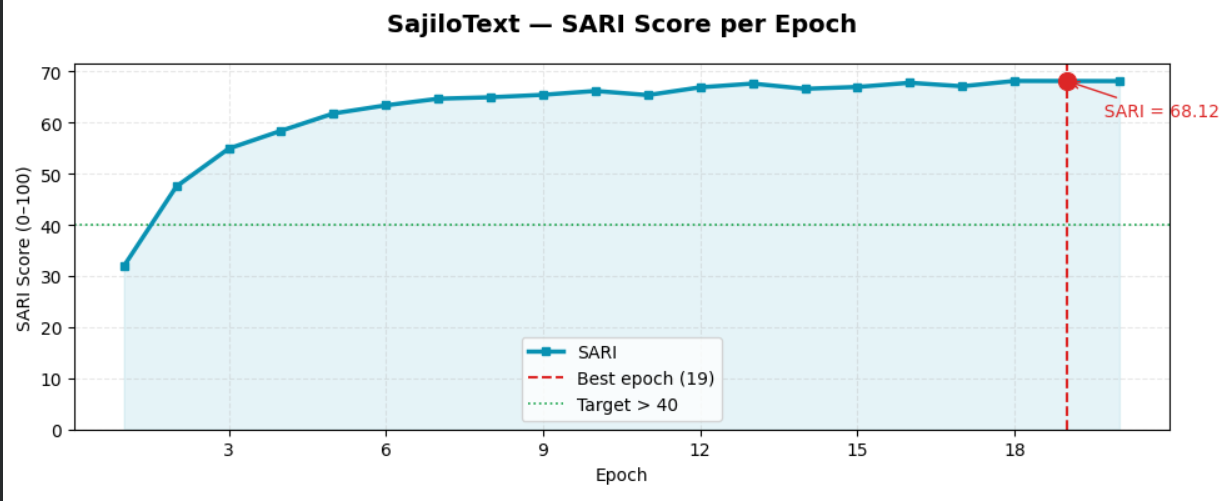
\includegraphics[width=0.8\textwidth]{sari.png}
    \caption{Sari Score each epoch}
    \label{fig:rouge_summary}
\end{figure}

\section{Discussion}

From the experimental results, it can be concluded that the proposed mT5-based approach performs effectively for Nepali legal text simplification. The BLEU score of \textbf{65.45} indicates strong agreement between the generated simplified text and the reference output. Similarly, the ROUGE scores confirm that the model preserves important information from the source text while rewriting it into a simpler form.

The loss curves demonstrate that the model converges in a stable manner without major oscillations. The gradual reduction in validation loss, together with the increase in BLEU score, suggests that the chosen training strategy is appropriate for the dataset. The performance stabilization after the middle epochs also indicates that the model learns the core simplification patterns early and then refines them in later stages.

Overall, these results show that the SajiloText system is capable of simplifying complex Nepali legal language with promising accuracy. The model is therefore suitable as a baseline system for legal Nepali text simplification and can be further improved in future work by using a larger dataset, stronger data cleaning, and more advanced decoding or evaluation strategies.

\chapter{Conclusion and Future Enhancement}

\section{Conclusion}

This project presented the design and implementation of a Nepali legal text simplification system using the multilingual Transformer model mT5. The main objective of the work was to transform complex and formal Nepali legal text into simpler Nepali while preserving the original legal meaning as much as possible. This objective is important because legal documents are often difficult for ordinary citizens, students, and non-expert readers to understand due to dense sentence structure, formal vocabulary, and the frequent use of conditions, restrictions, and exceptions.

To achieve this goal, the project focused on collecting Nepali legal text, cleaning and preprocessing the source material, constructing a parallel dataset of complex and simplified Nepali sentence pairs, and fine-tuning the mT5 model for the simplification task. Since Nepali legal simplification is a low-resource problem, dataset preparation became one of the most important contributions of the project. Special attention was given to maintaining high-quality simplification pairs so that the simplified output would be shorter, clearer, and easier to understand without changing the original intent of the legal sentence.

The project also demonstrated that Transformer-based models are suitable for this task because they can model long-range dependencies and contextual relationships more effectively than earlier rule-based or recurrent approaches. This is especially important in legal text, where the meaning of a sentence may depend on distant conditions such as exceptions, qualifiers, or legal references. By using mT5, the project benefited from multilingual pretraining and a text-to-text framework that is naturally aligned with the simplification problem.

The experimental workflow further highlighted the importance of preprocessing, parameter tuning, and output-quality control. Training a simplification model is not only a matter of fitting a neural network; it also requires careful handling of dataset structure, sentence segmentation, sequence length, decoding behavior, and quality evaluation. Through this process, the project established a practical foundation for Nepali legal text simplification and showed that it is possible to build a system that supports legal accessibility through natural language processing.

Overall, this project is significant in both practical and academic terms. Practically, it can help improve public understanding of legal language in Nepali. Academically, it contributes to the growing area of low-resource legal NLP by providing a structured dataset, a simplification pipeline, and a model development approach that can be extended in future work. The project therefore serves as a meaningful first step toward making Nepali legal information more accessible, understandable, and usable for a wider audience.

\section{Future Enhancement}

Although the project produced a working Nepali legal text simplification system, there are several areas in which it can be improved and extended in the future.

First, the dataset can be expanded significantly. The quality of a simplification model depends heavily on the variety and accuracy of the training data. In future work, the dataset can be enlarged beyond constitutional clauses to include other categories of Nepali legal text such as citizenship laws, public service rules, labor laws, tax procedures, court notices, administrative regulations, and citizen-facing legal documents. A larger and more diverse dataset would improve the generalization ability of the model and make the system more useful in real-world applications.

Second, future versions of the project can incorporate stronger quality-control mechanisms for simplification. At present, the model focuses on generating simpler Nepali text, but additional post-processing modules can be introduced to verify that legal meaning has not been altered. For example, a future system may include automatic checks for negation, conditions, dates, numbers, permissions, obligations, and prohibitions. Such a legal fidelity checking mechanism would make the system more reliable for practical use.

Third, the model architecture itself can be improved. While mT5-small is suitable for limited computational resources and project-level implementation, future work may explore larger models such as mT5-base or other encoder-decoder architectures. Parameter-efficient fine-tuning methods such as LoRA or adapter-based training can also be tested to improve performance while reducing hardware requirements. In addition, controlled text generation methods can be incorporated so that the user can choose different simplification levels, such as basic, moderate, or highly simplified output.

Fourth, the project can be extended beyond simplification alone. A future version may include difficult-word highlighting, legal vocabulary explanation, clause-wise explanation, and question-answering features. This would transform the system from a pure simplifier into a broader Nepali legal assistance tool. For instance, a citizen may submit a legal clause and receive not only a simpler version but also a list of difficult terms with plain Nepali meanings and a short explanation of the clause’s practical effect.

Fifth, evaluation can be improved further. In addition to BLEU and ROUGE scores, future work should include structured human evaluation involving legal experts, language experts, and general readers. Such evaluation can assess not only similarity to reference text but also readability, faithfulness, usefulness, and legal correctness. User studies with non-expert Nepali readers would also be valuable for measuring whether the system truly improves comprehension.

Sixth, future implementation can focus on deployment. The current project is primarily research-oriented, but the model can later be integrated into a web application, mobile application, or legal information portal. Such a deployment could provide an interface where users paste Nepali legal text and immediately receive a simpler version. This would significantly improve the practical impact of the work.

Finally, future research may explore multilingual or cross-lingual legal simplification in Nepali and English. Since many Nepali legal texts also exist in English translation, aligned bilingual resources may support stronger models, comparative experiments, and hybrid legal information systems. This would also open the possibility of legal text explanation, translation, and simplification across languages.

In summary, this project provides a solid foundation, but it also opens many promising directions for further research and development. With a larger dataset, stronger evaluation, legal fidelity controls, and practical deployment, the system can evolve into a highly useful tool for improving legal accessibility in Nepal.

\chapter{Web Application \& Demo}
% \addcontentsline{toc}{chapter}{\numberline{}Web Application \& Demo}
\subsection{Frontend Interface and Output Examples}

The developed \textbf{SajiloText} web interface allows users to input complex Nepali legal or governmental text and obtain a simplified version instantly. The interface is designed with two side-by-side panels: the left panel accepts the complex input text, while the right panel displays the simplified output generated by the model. Figures~\ref{fig:Image1}--\ref{fig:Image2} show sample outputs of the implemented system for different legal text inputs.

\begin{figure}[H]
    \centering
    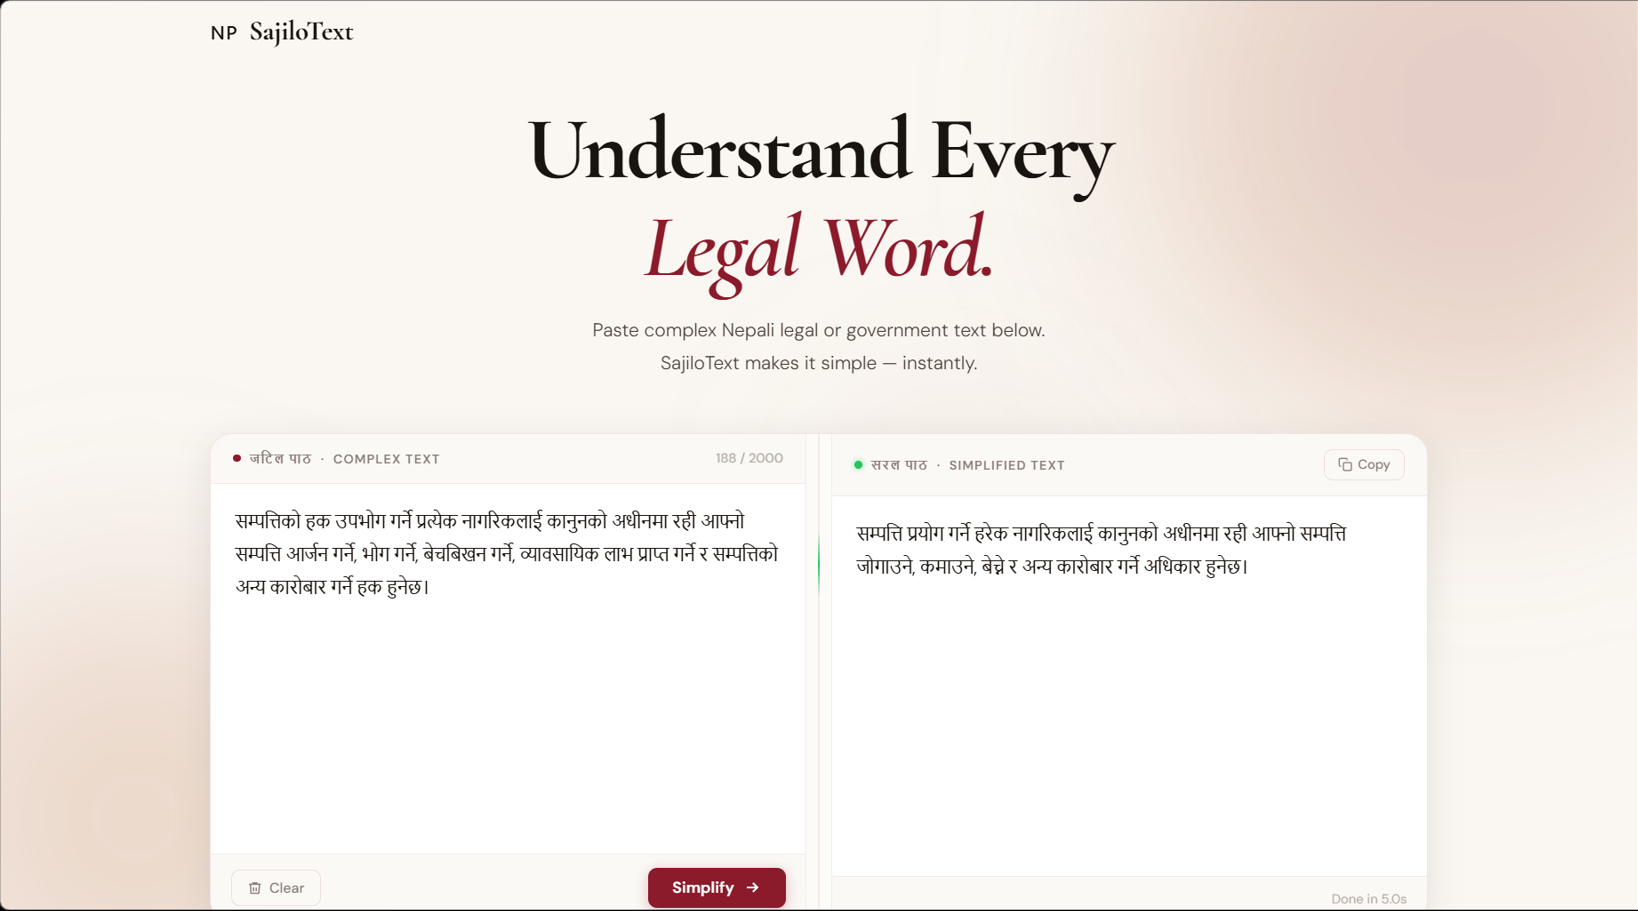
\includegraphics[width=\textwidth]{Screenshot 2026-03-19 093952.png}
    \caption{Text Simplification}
    \label{fig:Image1}
\end{figure}

\begin{figure}[H]
    \centering
    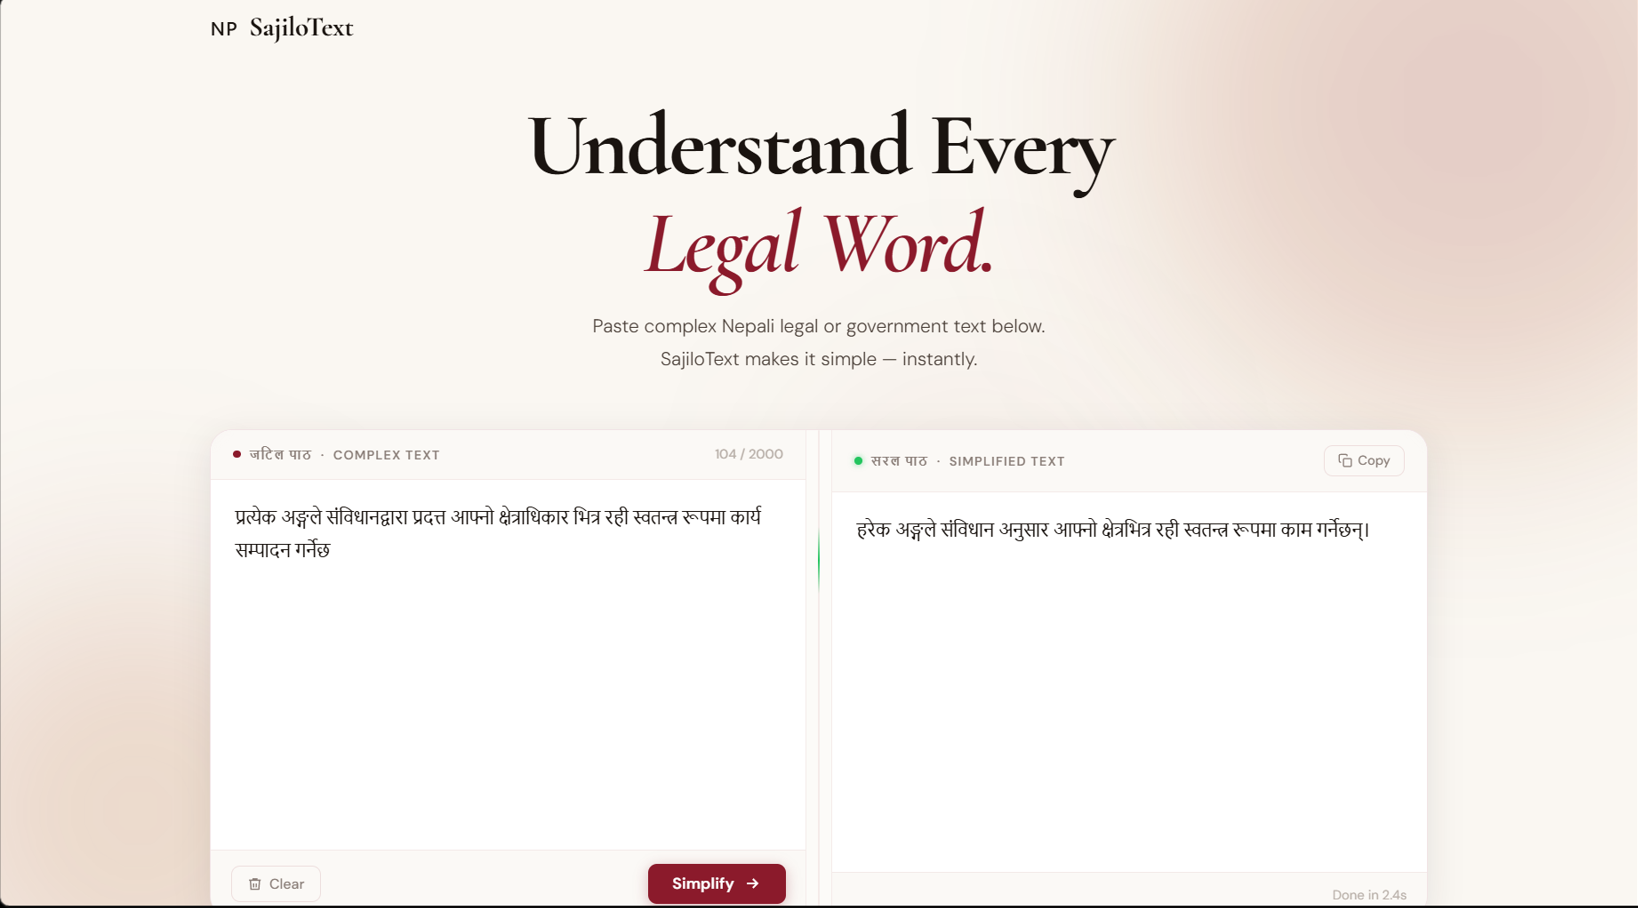
\includegraphics[width=\textwidth]{Screenshot 2026-03-19 094010.png}
    \caption{Text Simplification}
    \label{fig:Image2}
\end{figure}

\begin{figure}[H]
    \centering
    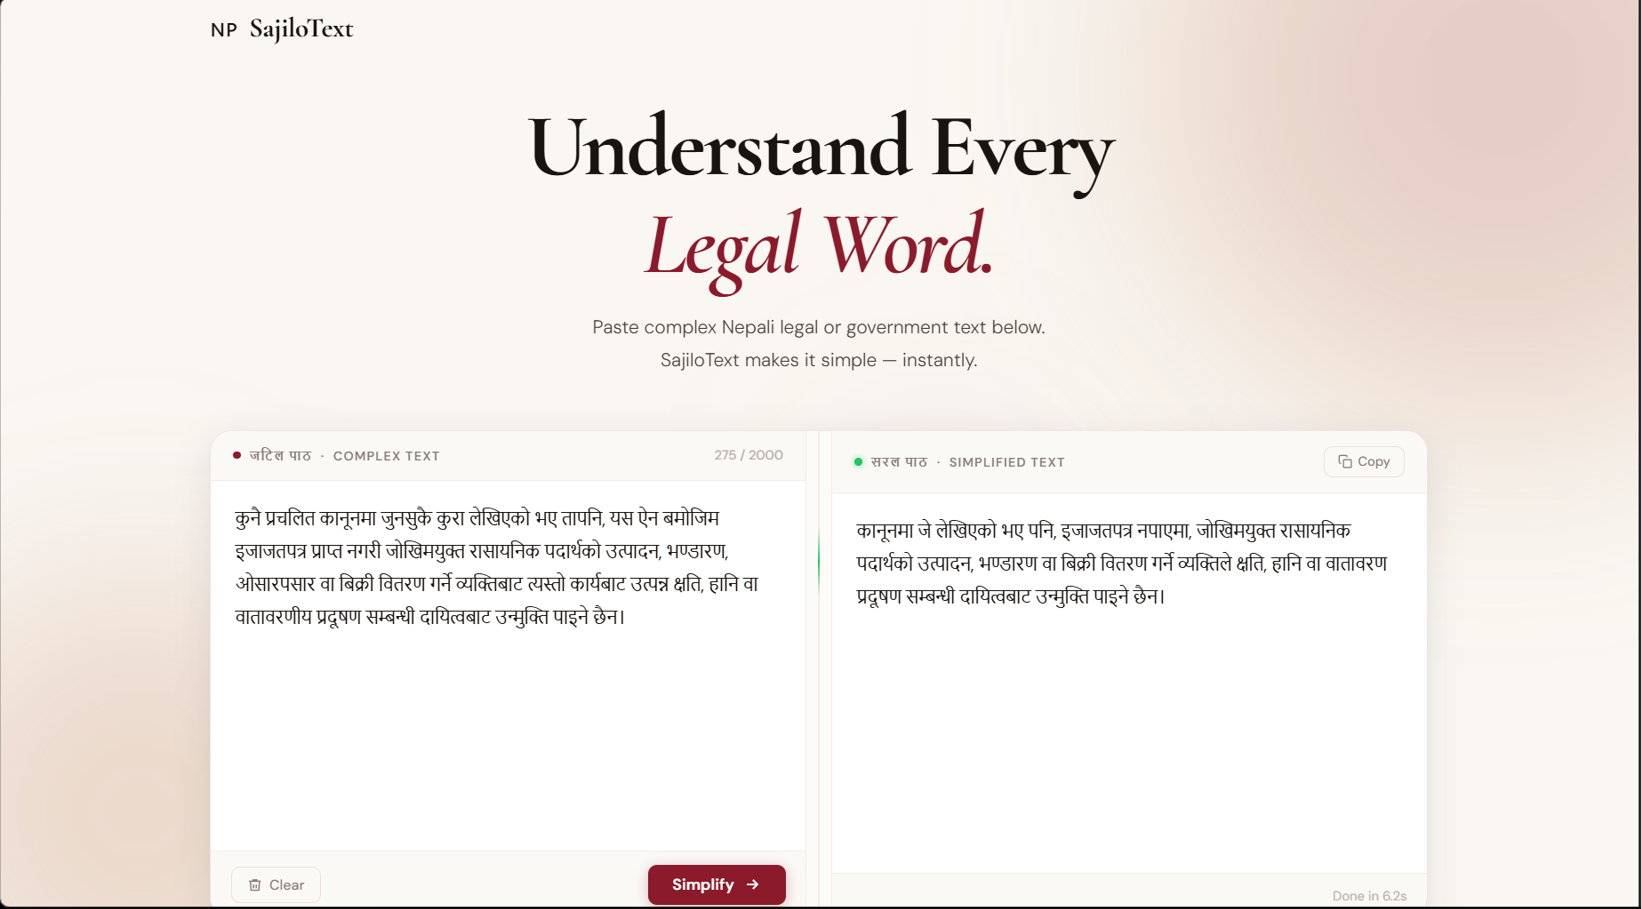
\includegraphics[width=\textwidth]{Screenshot 2026-03-19 094029.png}
    \caption{Text Simplification}
    \label{fig:Image3}
\end{figure}

---

% \chapter{Timeline}

% \begin{figure}[H]
% \centering
% \resizebox{0.95\textwidth}{!}{%
% \begin{ganttchart}[
%     hgrid,
%     vgrid,
%     x unit=0.9cm,
%     y unit title=0.7cm,
%     y unit chart=0.6cm,
%     bar height=0.5,
%     title height=1,
%     title label font=\scriptsize\bfseries,
%     bar label font=\scriptsize,
%     group label font=\scriptsize\bfseries,
%     milestone label font=\scriptsize,
%     progress label text={},
%     bar/.append style={fill=blue!40},
%     group/.append style={fill=orange!50},
%     milestone/.append style={fill=red!70, rounded corners=2pt}
% ]{1}{12}

% % ---- Title ----
% \gantttitle{\textbf{SajiloText Project Timeline (Oct 2024 -- Mar 2025)}}{12} \\
% \gantttitle{Oct '24}{2}
% \gantttitle{Nov '24}{2}
% \gantttitle{Dec '24}{2}
% \gantttitle{Jan '25}{2}
% \gantttitle{Feb '25}{2}
% \gantttitle{Mar '25}{2} \\

% % ---- Phases Only ----
% \ganttgroup[progress=100, group/.append style={fill=green!50}]{Phase 1: Planning \& Setup}{1}{3} \\
% \ganttgroup[progress=100, group/.append style={fill=green!50}]{Phase 2: Dataset Preparation}{3}{6} \\
% \ganttgroup[progress=60, group/.append style={fill=yellow!60}]{Phase 3: Model Development}{5}{9} \\
% \ganttgroup[progress=55, group/.append style={fill=yellow!60}]{Phase 4: System Integration}{6}{11} \\
% \ganttgroup[progress=0, group/.append style={fill=gray!40}]{Phase 5: Validation \& Testing}{11}{12} \\
% \ganttgroup[progress=0, group/.append style={fill=gray!40}]{Phase 6: Documentation}{11}{12} \\

% % ---- Milestones ----
% \ganttmilestone[milestone/.append style={fill=green!70}]{Dataset Ready}{6} \\
% \ganttmilestone[milestone/.append style={fill=yellow!70}]{Model Training Complete}{9} \\
% \ganttmilestone[milestone/.append style={fill=orange!70}]{System Integration Complete}{11} \\
% \ganttmilestone[milestone/.append style={fill=red!70}]{Project Submission}{12} \\

% \end{ganttchart}
% }
% \caption{Simplified Gantt Chart of the Project Phases}
% \label{fig:gantt}
% \end{figure}

% \vspace{1em}
% \begin{flushright}
% \setlength{\fboxsep}{1pt}
% \begin{tabular}{r l}
% \textcolor{green!60}{\rule{10pt}{10pt}} & \textbf{Completed} \\[3pt]
% \textcolor{yellow!60}{\rule{10pt}{10pt}} & \textbf{In Progress} \\[3pt]
% \textcolor{gray!50}{\rule{10pt}{10pt}} & \textbf{Upcoming} \\[3pt]
% \textcolor{red!70}{\rule{10pt}{10pt}} & \textbf{Final Milestone } \\
% \end{tabular}
% \end{flushright}







% \chapter{References}
% \addcontentsline{toc}{chapter}{\numberline{}References}




\cleardoublepage
\phantomsection
\addcontentsline{toc}{chapter}{Bibliography}

\begin{thebibliography}{99}

\bibitem{bal2010}
Bal, B. K., \& Rupakheti, P. (2010).
Developing a Nepali National Corpus.
\textit{Proceedings of the Eighth Workshop on Asian Language Resources}.

\bibitem{chalkidis2020}
Chalkidis, I., Fergadiotis, M., Malakasiotis, P., Aletras, N., \& Androutsopoulos, I. (2020).
LEGAL-BERT: The muppets straight out of law school.
\textit{Proceedings of the 2020 Conference on Empirical Methods in Natural Language Processing: Findings}.

\bibitem{kudo2018}
Kudo, T., \& Richardson, J. (2018).
SentencePiece: A simple and language independent subword tokenizer and detokenizer for neural text processing.
\textit{Proceedings of EMNLP 2018}.

\bibitem{lin2004}
Lin, C. Y. (2004).
ROUGE: A package for automatic evaluation of summaries.
\textit{Text Summarization Branches Out, Workshop at ACL 2004}.

\bibitem{martin2020}
Martin, L., Fan, A., Bordes, A., Joulin, A., \& Sagot, B. (2020).
Multilingual unsupervised sentence simplification.
\textit{arXiv preprint arXiv:2005.00352}.

\bibitem{nisioi2017}
Nisioi, S., Stajner, S., Ponzetto, S. P., \& Dinu, L. P. (2017).
Exploring neural text simplification models.
\textit{Proceedings of the 55th Annual Meeting of the Association for Computational Linguistics}.

\bibitem{papineni2002}
Papineni, K., Roukos, S., Ward, T., \& Zhu, W. J. (2002).
BLEU: A method for automatic evaluation of machine translation.
\textit{Proceedings of ACL 2002}.

\bibitem{raffel2020}
Raffel, C., Shazeer, N., Roberts, A., et al. (2020).
Exploring the limits of transfer learning with a unified text-to-text transformer.
\textit{Journal of Machine Learning Research}, 21(140), 1--67.

\bibitem{scarton2018}
Scarton, C., \& Specia, L. (2018).
Learning simplifications for specific target audiences.
\textit{Proceedings of ACL 2018}.

\bibitem{sheang2021}
Sheang, K. C., \& Saggion, H. (2021).
Controllable sentence simplification with a unified text-to-text transfer transformer.
\textit{Proceedings of the International Conference on Recent Advances in Natural Language Processing}.

\bibitem{siddharthan2006}
Siddharthan, A. (2006).
Syntactic simplification and text cohesion.
\textit{Research on Language \& Computation}, 4(1), 77--109.

\bibitem{sutskever2014}
Sutskever, I., Vinyals, O., \& Le, Q. V. (2014).
Sequence to sequence learning with neural networks.
\textit{Advances in Neural Information Processing Systems (NeurIPS 2014)}.

\bibitem{vaswani2017}
Vaswani, A., Shazeer, N., Parmar, N., et al. (2017).
Attention is all you need.
\textit{Advances in Neural Information Processing Systems 30 (NeurIPS 2017)}.

\bibitem{xu2015}
Xu, W., Callison-Burch, C., \& Napoles, C. (2015).
Problems in current text simplification research: New data can help.
\textit{Transactions of the Association for Computational Linguistics}, 3, 283--297.

\bibitem{xue2021}
Xue, L., Constant, N., Roberts, A., et al. (2021).
mT5: A massively multilingual pre-trained text-to-text transformer.
\textit{Proceedings of NAACL 2021}.

\end{thebibliography}

% \chapter{Appendix A: Sample Dataset Entry}
% \begin{verbatim}
% {
%   "id": "001",
%   "difficulty": "A",
%   "original_nepali": "संविधानले नागरिकलाई प्रदान गरेका 
%   मौलिक अधिकारहरू अनुल्लंघनीय छन्।",
%   "simplified_nepali": "संविधानले दिएका मुख्य अधिकारहरू 
%   कसैले पनि खोस्न सक्दैन।",
%   "vocabulary": {
%     "मौलिक": "मुख्य, आधारभूत",
%     "अनुल्लंघनीय": "खोस्न नसकिने, उल्लंघन गर्न नमिल्ने"
%   },
%   "english_translation": "The fundamental rights granted 
%   by the constitution to citizens cannot be violated."
% }
% \end{verbatim}

% \chapter{Appendix B: User Interface Mockups}
% \begin{figure}[H]
% \centering
% \begin{tikzpicture}
% % Main container
% \draw[thick] (0,0) rectangle (12,8);
% % Header
% \draw[fill=blue!20] (0,7) rectangle (12,8);
% \node at (6,7.5) {\Large \textbf{SajiloText - Nepali Text Simplifier}};
% % Input section
% \draw (0.5,5.5) rectangle (11.5,6.8);
% \node[anchor=west] at (0.7,6.5) {\textbf{Input Text or Upload Image:}};
% \draw (1,5.7) rectangle (11,6.3);
% \node at (6,6) {Enter Nepali text here...};
% % Button
% \draw[fill=green!30] (5,5) rectangle (7,5.4);
% \node at (6,5.2) {\textbf{Simplify}};
% % Output sections
% \draw (0.5,0.5) rectangle (5.5,4.5);
% \node[anchor=north] at (3,4.3) {\textbf{Simplified Nepali}};
% \draw (6.5,0.5) rectangle (11.5,4.5);
% \node[anchor=north] at (9,4.3) {\textbf{English Translation}};
% \end{tikzpicture}
% \caption{Web Interface Mockup}
% \end{figure}

% \chapter{Appendix C: Evaluation Rubric}
% \begin{table}[H]
% \centering
% \begin{tabular}{|l|p{10cm}|}
% \hline
% \textbf{Criteria} & \textbf{Description} \\
% \hline
% Semantic Preservation & Does the simplified text maintain the original meaning? (1-5) \\
% \hline
% Readability & Is the simplified text easier to understand? (1-5) \\
% \hline
% Grammatical Correctness & Is the simplified text grammatically correct? (1-5) \\
% \hline
% Vocabulary Simplification & Are complex words replaced with simpler alternatives? (1-5) \\
% \hline
% Overall Quality & Overall assessment of the output (1-5) \\
% \hline
% \end{tabular}
% \caption{Human Evaluation Rubric}
% \end{table}
\end{document}